\documentclass{article}

\usepackage[utf8]{inputenc}
\usepackage[T1]{fontenc}
\usepackage{geometry}
\usepackage{xcolor}
\usepackage{graphicx}
\usepackage{subcaption}
\usepackage{verbatim}
\usepackage{amsmath,amssymb}
\usepackage{amstext}
\usepackage{amsthm}
\usepackage{steinmetz}
\usepackage{stackrel}
\usepackage{mathtools}
\newcommand{\angstrom}{\text{\normalfont\AA}}
\usepackage{hyperref}


\geometry{a4paper}

\usepackage[english]{babel}
\frenchspacing

\hypersetup{
  colorlinks=true,
  linkcolor = black,
}


\title{Electronics laboratory report - calculator}
\author{Lorenzo Ramella, Alessandro Matteo Rossi, Marco Tambini}
\date{June 10, 2021}


\begin{document}
\maketitle

\begin{abstract}
  The goal of this project is creating a calculator able to perform addition and subtractions by using logic gates.

\vspace{3mm}

  We created two different circuits: a 3-bit real calculator created in laboratory, and a 16-bit simulated calculator, to show how it is possible to solve the issue of the increasing complexity due to the size growth. Most of the used circuits have been both simulated and created in laboratory.

\vspace{3mm}

  The circuital simulator used is "circuitjs1". %scusaci stef ma siamo poveri, tu c'hai lo smartwatch e lo flexavi l'ultima volta in lab
\end{abstract}
\clearpage
\tableofcontents

\clearpage

\section{Basics concepts}

\subsection{Boolean algebra}
To make calculations, a circuit needs to be able to perform logical operations. In particular, we usually use boolean algebra in digital electronics. 

\vspace{3mm}

To be able to create a circuit like this, first of all, we need to define the various components.
The number 0 and 1 need to be properties of an electrical circuit that can be "moved" and they can be realized using voltage. We can assign the number 0 to a low voltage and the number 1 to a high voltage. 

\vspace{3mm}

For example, if we define $0\,\textrm{V}$ as low, negative or 0 and $5\,\textrm{V}$ as high, positive or 1, we can define a threshold voltage exactly in the middle, so that any voltage under $2.5\,\textrm{V}$ will be considered 0, and any voltage above it will be considered 1.

\vspace{3mm}

Once 1 and 0 are defined, we need to define the operations that can be performed:

\begin{itemize}
\item $"!"$ is the negation, and it can be represented by a NOT gate.
\item $"+"$ is the addition, and it can be represented by an OR gate.
\item $"*"$ is the multiplication, and it can be represented by an AND gate.
\end{itemize}



\subsection{Classical operations in boolean algebra}

\subsubsection{Addition and subtraction}

In order to sum up two binary numbers, we perform a classical column sum, keeping track of the carry-overs.

\vspace{5mm}

Subtracting two binary numbers is slightly more difficult. We point out that, if we consider a binary number $A$, its opposite is
\[-A=NOT(A)+1\]

This means that a subtraction can be performed by summing up a first number $X_1$ and the opposite of the second number $-X_2$. 

\vspace{3mm}

In our project we will use a ripple carry adder, that will be presented in section \ref{RCA_Section}. This component is able to sum $X_1$ with the opposite of $X_2$ and then it will add "1". This is possible thanks to the commutative property.

\vspace{3mm}

Now let's perform a subtraction among $6$ and $3$, which respectively correspond to $0110$ and $0011$. First of all we do
\[0110+NOT(0011) = 0110 + 1100 = (1)0010\]

We leave the last carry-over, if present like in this case, because inputs and output must have the same amount of binary digits.

Then we add "1"

\[(1)0010+1=(1)0011 = 0011\]
  
And this is equal to 3 in decimal form.



\subsubsection{Multiplication}

In order to multiply two binary numbers, you need to subdivide the operation in different phases. The second factor has to be split into numbers with a single "1" bit, and the first factor is multiplied to every single division. Then the results are summed up. The multiplication is a classical multiplication among real numbers. 

\vspace{3mm}

For example let's take $6 \cdot 10$, which is $0110 \cdot 1010$ in binary form. If we subdivide the multiplication in $0110 \cdot 1000$ and $0110 \cdot 0010$, we can simply add up all these results. The result is $110000 + 001100 = 111100$ which corresponds with 60 in decimal form. We specify that the multiplication by 10 is seen as a multiplication by 8 summed to a multiplication by 2.












\section{Logic gates}

When we talk about a logic gate, we are describing a circuit that can take a certain number of inputs and gives a single output, depending on the input received. The output needs to be readable by another logic gate of the same family.

\vspace{3mm}

The main logic gates are the following, represented with their circuital symbol in figure \ref{LogicGates}.

\begin{figure}[h!]

    \centering
    \begin{subfigure}{.4\textwidth}
        \centering
        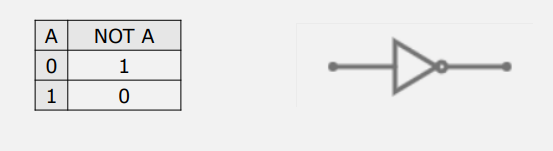
\includegraphics[width=\linewidth]{IM_NOT.PNG}
        \caption{NOT gate}
        \label{NOT}
    \end{subfigure}
    \hfill
    \begin{subfigure}{.4\textwidth}
        \centering
        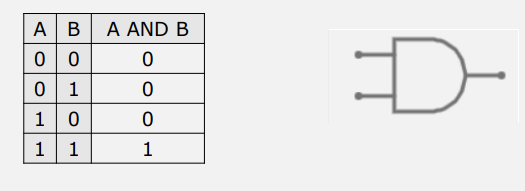
\includegraphics[width=\linewidth]{IM_AND.PNG}
        \caption{AND gate}
        \label{AND}        
    \end{subfigure}
    
    \centering
    \begin{subfigure}{.4\textwidth}
        \centering
        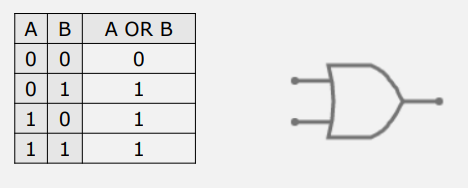
\includegraphics[width=\linewidth]{IM_OR.PNG}
        \caption{OR gate}
        \label{OR}
    \end{subfigure}
    \hfill
    \begin{subfigure}{.4\textwidth}
        \centering
        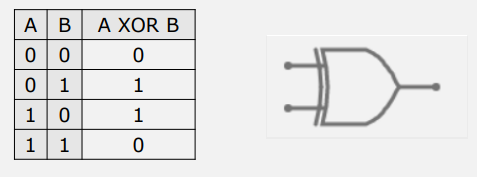
\includegraphics[width=\linewidth]{IM_XOR.PNG}
        \caption{XOR gate}
        \label{XOR}        
    \end{subfigure}
    
    \centering
    \begin{subfigure}{.4\textwidth}
        \centering
        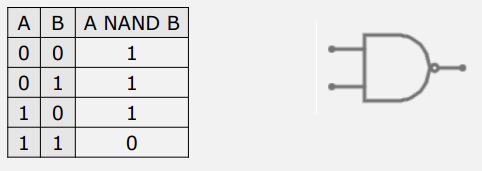
\includegraphics[width=\linewidth]{IM_NAND.PNG}
        \caption{NAND gate}
        \label{NAND}
    \end{subfigure}
    \hfill
    \begin{subfigure}{.4\textwidth}
        \centering
        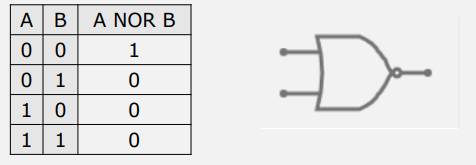
\includegraphics[width=\linewidth]{IM_NOR.PNG}
        \caption{NOR gate}
        \label{NOR}        
    \end{subfigure}
    
    \centering
    \begin{subfigure}{.4\textwidth}
        \centering
        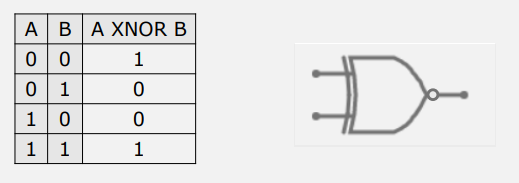
\includegraphics[width=\linewidth]{IM_XNOR.PNG}
        \caption{XNOR gate}
        \label{XNOR}
    \end{subfigure}

\caption{Image of the main logic gates used in digital electronics}
\label{LogicGates}
\end{figure}




\clearpage

\subsection{N-MOS}

In order to create these logic gates, we need to know how to use a MOSFET. For this project we used N-MOS transistors only.

\vspace{3mm}

The N-MOS is a transistor that gets as input a gate voltage, a drain voltage, a source voltage and a body voltage. In most cases the source and the body are internally connected, since the body needs to be at the lowest voltage and the source is usually grounded.

\vspace{3mm}

When a positive voltage is applied between the drain and source, a deplition layer that blocks the current flow is formed. 
If we then start applying a positive voltage between gate and body, the electrons will start "balancing" the gaps in the P substrate, but the current will still be zero.

\vspace{3mm}

After $V_{GS}$ (the potential difference among gate and source) overcomes a certain threshold voltage, the current will start to flow from drain to source. At the beginning of this flow, the ratio between the current and $V_{DS}$ (the potential difference among drain and source) is linear but, when $V_{DS}$ becomes big enough, the function becomes almost constant (see figure \ref{NMOS_Function}) and we find ourself in the saturation region.

\begin{figure}[h]
    \centering
    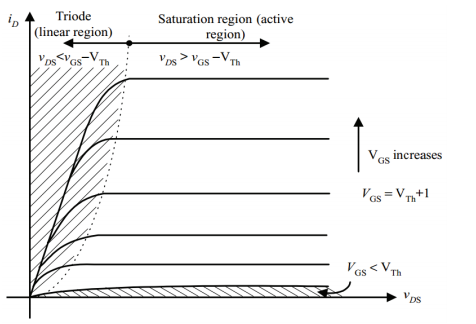
\includegraphics[scale=.65]{IM_NMOS_Function.png}
    \caption{Graph of the I-V N-MOS function}
    \label{NMOS_Function}
\end{figure}

\vspace{3mm}

We do not need to distinguish linear section and saturation section, as we will check only the voltage at the drain of the N-MOS for our gate. The threshold voltage is different for every transistor, and it usually is within the range $0.5\,\textrm{V} - 5\,\textrm{V}$. The transistor we used is the $IRF822$, whose threshold voltage has been measured in lab, and it is approximately $3 \,\textrm{V}$ (calculated from a laboratory measure with no statistical analysis done, but backed up by the values reported on the datasheet). We decided to use $5\,\textrm{V}$ for $V_{GS}$ to make input and output approximately the same, as we will see later.


\clearpage


\subsection{NOT gate}

The easiest logic gate to realize is the NOT gate. We remember that the NOT gate negates the only input it receives. We need a high enough resistance and one N-MOS (as represented in figure \ref{NOT_N-MOS}) to realize it.

\begin{figure}[h]
    \centering
    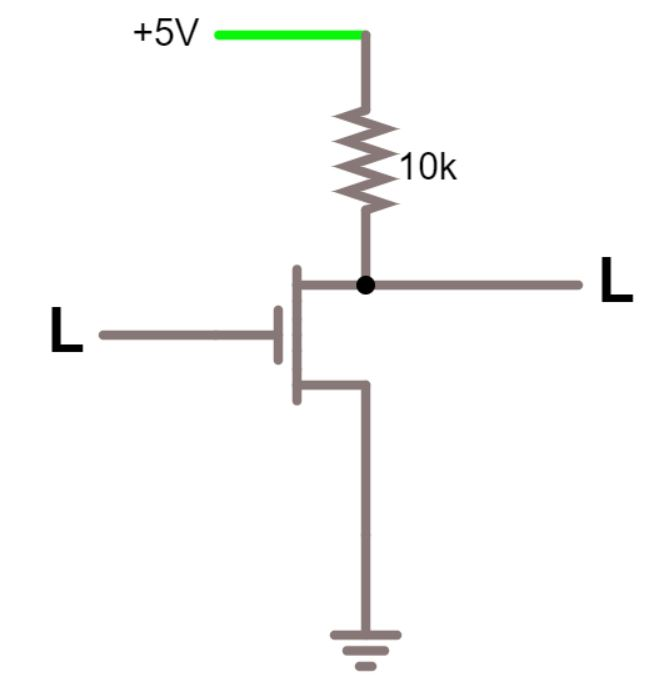
\includegraphics[scale=0.3]{IM_NOT_NMOS.JPG}
    \caption{NOT logic gate realized using a N-MOS and a resistor}
    \label{NOT_N-MOS}
\end{figure}

When the input is 0, the N-MOS will not let the current flow and, thanks to Ohm First Law, we know that the voltage drop across the resistor should be 0, so we get the same supply voltage. The read output will be around $5\,\textrm{V}$, so we get a 1 as output.

\vspace{3mm}

When the input is 1, the N-MOS will let the current flow with a small resistance value. Since there is a higher resistance before the N-MOS, almost all the voltage drop will occur on the previous one, and the drain will be almost zero. The read output will be around $0\,\textrm{V}$, so we get a 0 output.

\vspace{3mm}

With this configuration the signal will not be properly negated for high frequencies, and it will be like in the last picture in figure \ref{ResistiveInverter} (it will never reach a 1 state).

A possible solution consists of a combination of N-MOS and P-MOS but, since our calculator does not have to work at such high frequencies, we dismissed this problem.

\begin{figure}[h]
    \centering
    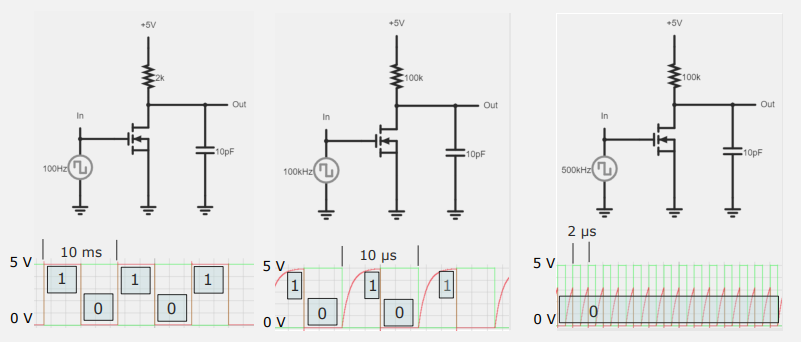
\includegraphics[scale=0.6]{IM_inverter_esa.PNG}
    \caption{Inverter N-MOS circuit with a resistive load}
    \label{ResistiveInverter}
\end{figure}

For the picture of the NOT gate realized in laboratory check figure \ref{NOT_LAB} in Appendix.


\clearpage
\subsection{NOR gate}

Once we created the NOT gate, we proceeded to realize the NOR gate since, as we will explain later in Section \ref{OtherGates}, the NOR and the NAND gate are both functional complete.

\vspace{1mm}

The NOR gate is composed, as seen in figure \ref{NOR_N-MOS}, by two NOT gates short-circuited at their output.

\begin{figure}[h]
    \centering
    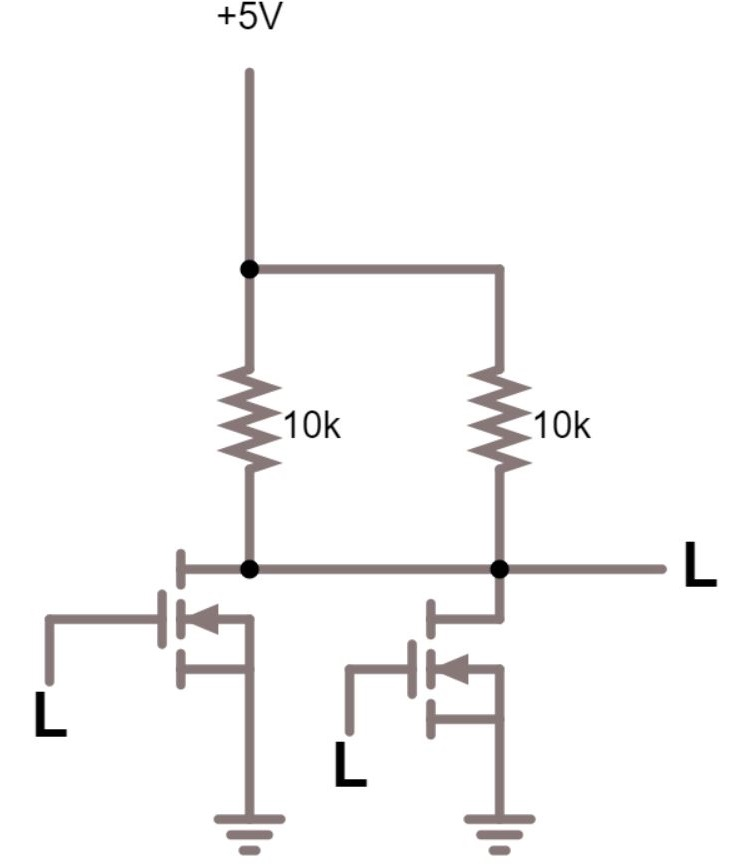
\includegraphics[scale=.3]{IM_NOR_NMOS.JPG}
    \caption{NOR logic gate realized using two short-circuited NOT gates}
    \label{NOR_N-MOS}
\end{figure}

When both inputs are 0, the two N-MOS will not let any current pass and, just like in the NOT gate, the output will be 1.

\vspace{1mm}

When one or both inputs are 1 the N-MOS will let the current flow and there will be a voltage drop across the resistor. So the output will be 0.

\vspace{1mm}

The role of the short circuit is ensuring that whether an input is positive, the current will pass through the "open" N-MOS.

\vspace{3mm}

For the picture of the NOR gate realized in laboratory check figure \ref{NOR_LAB} in Appendix.



\subsection{NAND gate}

As we said for the NOR gate, the NAND gate is also functional complete. But it can be created without the shortcircuit needed by the NOR gate, so it is slightly cheaper. 

\vspace{3mm}

The NAND gate is realized with a series resistor followed by two N-MOS, where the source of the first is plugged in the drain of the second, as seen in figure \ref{NAND_NMOS}.

\begin{figure}[h]
    \centering
    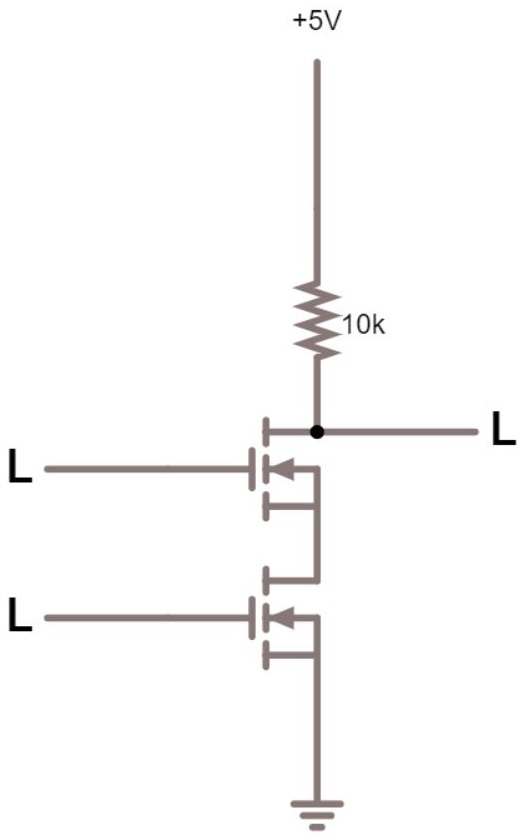
\includegraphics[scale=.25]{IM_NAND_NMOS.JPG}
    \caption{NAND gate realized with one resistor and two N-MOS transistors}
    \label{NAND_NMOS}
\end{figure}

\vspace{3mm}

When both inputs are 1, the current will be able to flow and the output will be 0.

\vspace{1mm}

When one of the inputs is 0, one of the N-MOS will be "closed" and, since the current cannot pass, the output will be 1.

\vspace{3mm}

For the picture of the NAND gate realized in laboratory check figure \ref{NAND_LAB} in Appendix.



\subsection{Other logic gates} \label{OtherGates}

Being functional complete means that a single logic gate can be the only component in a circuit, and that circuit will be equivalent to any other logic gate. NAND and NOR gates have this property (see figure \ref{NAND_allpowerful} and \ref{NOR_allpowerful} in appendix).

\vspace{3mm}

The only gates needed for the calculator are shown in figure \ref{UsefulGates}, and they are: 

\begin{itemize}
\item The AND gate, made by the NAND gate, where the output is negated by a NOT.
\item The OR gate, made by the NOR gate, where the output is negated by a NOT.
\item The XOR gate, made by four NAND gates as shown in figure \ref{XOR_NANDs}
\end{itemize}

\begin{figure}[h]
    \centering
    \begin{subfigure}{.49\textwidth}
        \centering
        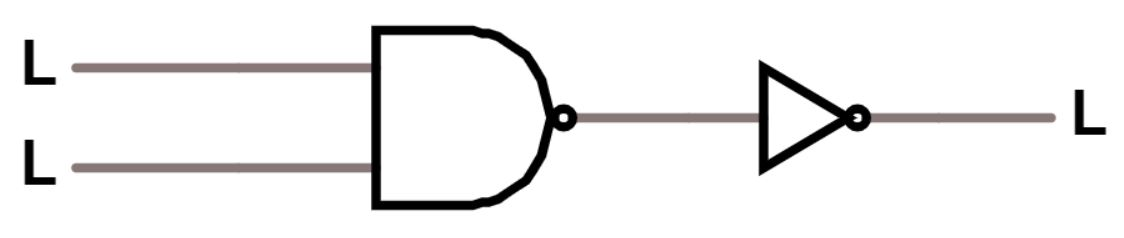
\includegraphics[scale=.3]{IM_AND_LOGIC.JPG}
        \caption{AND gate built using a negated NAND gate}
    \end{subfigure}
    \hfill
    \begin{subfigure}{.49\textwidth}
        \centering
        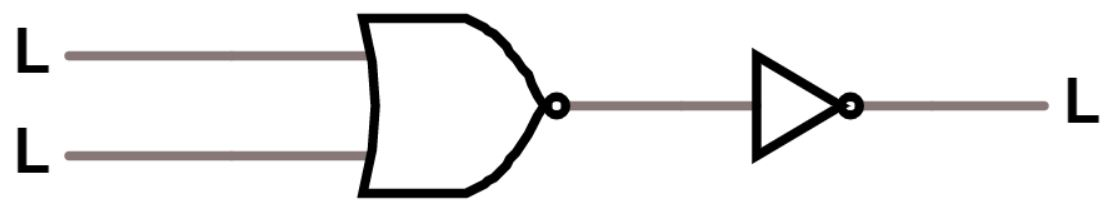
\includegraphics[scale=.3]{IM_OR_LOGIC.JPG}
        \caption{OR gate built using a negated NOR gate}       
    \end{subfigure}
    \vspace{2mm}
    \begin{subfigure}{\textwidth}
        \centering
        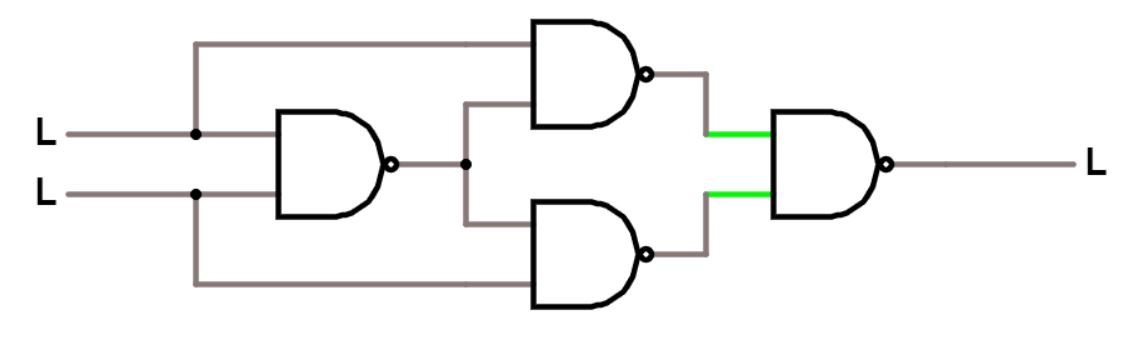
\includegraphics[scale=.3]{IM_XOR_LOGIC.JPG}
        \caption{XOR gate built using a four NAND gates}     
        \label{XOR_NANDs}     
    \end{subfigure}
    \caption{The logic gates used in the calculator}
    \label{UsefulGates}
\end{figure}
\clearpage
\subsection{Bistable circuit}

For the 16-bit calculator, that will be discussed in section \ref{SimulatedCalculator}, we also needed to be able to store information.

\vspace{1mm}

This means that we need a component that will work as memory. It has to be able to get an input and keep it saved as long as necessary, even if the input signal has already expired. Since the memory has to be both writable and readable, it needs a second input line to clear it.

\vspace{3mm}

The circuit that corresponds to the memory we need is the bistable circuit, also known as flip-flop (shown in figure \ref{FlipFlop}).

\begin{figure}[h]
    \centering
    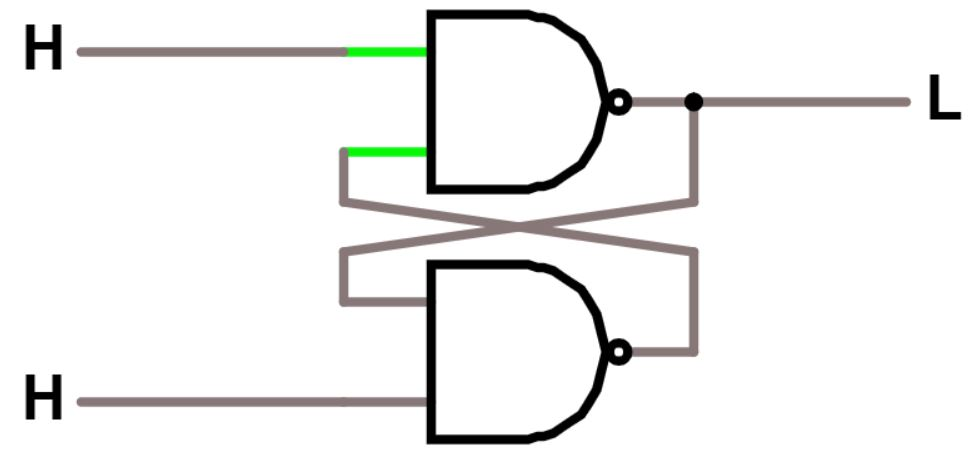
\includegraphics[scale=.3]{IM_FlipFlop}
    \caption{The circuit used to create a flip-flop memory unit}
    \label{FlipFlop}   
\end{figure}

The flip-flop can be created by both NOR gates and NAND gates but, since the NAND gates are cheaper, we decided to use those. This meant that the input has to be negated in order to work properly. Flip-flop truth table can be found in table \ref{FlipFlopTT}.


\begin{table}[h]
\centering
\begin{tabular}{ | c | c  c  c | c  c |}
\hline
 \# & $Set$ & $Clear$ & $Old Q$ & $New Q$ & $New Q'$\\
\hline
 \ 1 & 0 & 0 & 0 & 1 & 1 \\ 
 \ 2 & 0 & 0 & 1 & 1 & 1 \\
\hline 
 \ 3 & 0 & 1 & 0 & 1 & 0 \\ 
 \ 4 & 0 & 1 & 1 & 1 & 0 \\ 
 \ 5 & 1 & 0 & 0 & 0 & 1 \\
 \ 6 & 1 & 0 & 1 & 0 & 1 \\
\hline
 \ 7 & 1 & 1 & 0 & 0 & 1 \\
 \ 8 & 1 & 1 & 1 & 1 & 0 \\ 
\hline
\end{tabular}
\caption{Flip-flop truth table. Please note that the first two rows are not ideal for the storage of data, as $Q$ and $Q'$ have the same value. Rows 3-6 represent the moment when an input is given, whereas 7 and 8 is when data is stored.}
\label{FlipFlopTT}
\end{table}

\clearpage
\section{Encoder}

While calculators work using binary numbers, this kind of numeration is unfamiliar and difficult to use for most humans. This is why it is worth to develop an encoder, a circuit that converts decimal inputs in binary numbers.

\subsection{Simple encoder}

\begin{figure}[h]
  \centering
  %\captionsetup{justification=centering,margin=2cm}
  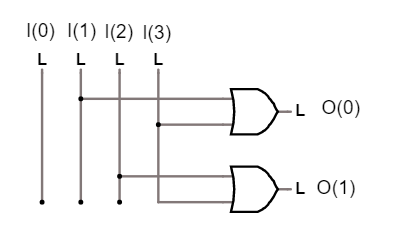
\includegraphics[scale=0.7]{simple_encoder}
  \caption{A simple encoder}
  \label{simple_encoder}
\end{figure}

A simple encoder is the easiest possible design for an encoder. There are $2^n$ input lines, and $n$ OR gates. When one of the input lines gets high voltage, it activates the OR gates corresponding to its binary representation.

\begin{table}[h]
  \centering
  \begin{tabular}{| c | c | c | c || c | c |}
  \hline
  I$_0$ & I$_1$ & I$_2$ & I$_3$ & O$_1$ & O$_0$ \\ \hline
  0 & 0 & 0 & 0 & 0 & 0 \\ \hline
  1 & 0 & 0 & 0 & 0 & 0 \\ \hline
  0 & 1 & 0 & 0 & 0 & 1 \\ \hline
  0 & 0 & 1 & 0 & 1 & 0 \\ \hline
  0 & 0 & 0 & 1 & 1 & 1 \\ \hline
  \end{tabular}
  \caption{Truth table for the 2-bit simple encoder}
  \label{Table_simple_encoder}
\end{table}

This circuit implementation is very simple, but it does not return a correct result if more than one input line is high. In such cases, it is advisable to use a priority encoder.

\clearpage

\subsection{Priority encoder} \label{PriorityEncoderSection}

\begin{figure}[h]
  \centering
  %\captionsetup{justification=centering,margin=2cm}
  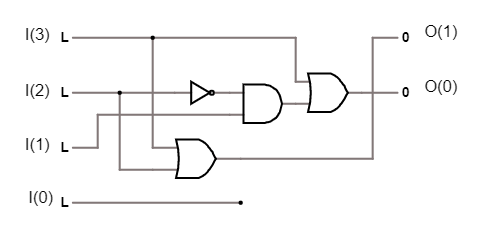
\includegraphics[scale=0.7]{priority_encoder}
  \caption{A priority encoder}
  \label{priority_encoder}
\end{figure}

A priority encoder is similar to a simple encoder, but it works even if more lines are high at the same time, giving priority to the highest number. It achieves this results by using AND gates: the OR gate inputs are no longer directly connected to the input lines, but they need to be "checked" by an AND gate. The AND gate receives as inputs the corresponding input line and the negation of any input line which:

\begin{itemize}
\item has an value higher than the first input line;
\item its binary representation is 0 in that position.
\end{itemize}

This way, each input line not only activates the OR gates corresponding to its binary representation, but also de-activates the ``wrong'' OR gates that a lower value input line could activate.

\vspace{3mm}

An example of how this works is provided in figure \ref{priority_encoder}. When $I(2)$ is low, the AND gate has the same value of $I(1)$, and the circuit works like a simple encoder; when $I(2)$ is high, the AND gate is always low, no matter the value of $I(1)$.

\begin{table}[h]
  \centering
  \begin{tabular}{| c | c | c | c || c | c |}
  \hline
  I$_0$ & I$_1$ & I$_2$ & I$_3$ & O$_0$ & O$_1$ \\ \hline
  x & 0 & 0 & 0 & 0 & 0 \\ \hline
  x & 1 & 0 & 0 & 1 & 0 \\ \hline
  x & x & 1 & 0 & 0 & 1 \\ \hline
  x & x & x & 1 & 1 & 1 \\ \hline
  \end{tabular}
  \caption{Truth table for the 2-bit priority encoder}
  \label{Table_priority_encoder}
\end{table}

\clearpage









\section{Processing}

In order to create a calculator that could perform additions and subtractions, we needed to have a component able to sum (or subtract) two binary numbers.

\subsection{Half adder and full adder}

The easiest component that can do this task is the half adder. It is a small circuit with 2 inputs and two outputs, and it is capable of summing up two binary digits. The input are the two digits, and the outputs are the sum $S$, performed by a XOR gate (which truth table is in figure \ref{XOR}), and the carry-over $C$, calculated by an AND gate (which truth table is in figure \ref{AND}).

\vspace{3mm}

Half adder truth table can be found in table \ref{HalfAdderTT}.

\begin{table}[h]
  \centering
  \begin{tabular}{| c | c || c | c |}
  \hline
  A$_1$ & A$_2$ & S & C \\ \hline
  0 & 0 & 0 & 0 \\ \hline
  1 & 0 & 1 & 0 \\ \hline
  0 & 1 & 1 & 0 \\ \hline
  1 & 1 & 0 & 1 \\ \hline
  \end{tabular}
  \caption{Half adder truth table, where $A_1$ and $A_2$ are the input bits, $S$ is the result, and $C$ the carry-over}
  \label{HalfAdderTT}
\end{table}

The major issue with this component is not being useful during a sum of two binary numbers. We specify that a sum of two binary numbers is a classical column sum. For this reason the half adder is not the best choice, because it cannot track the carry-over of the sum performed on the previous bit, if present.

\vspace{5mm}

If we want to sum two positive n-bit binary numbers, we need to keep track of the carry-overs. The right component for this duty is a full-adder, whose truth table can be found in table \ref{FullAdderTT}

\begin{table}[h]
  \centering
  \begin{tabular}{| c | c | c || c | c |}
  \hline
  A$_1$ & A$_2$ & C$_{in}$ & S & C$_{out}$ \\ \hline
  0 & 0 & 0 & 0 & 0 \\ \hline
  0 & 1 & 0 & 1 & 0 \\ \hline
  1 & 0 & 0 & 1 & 0 \\ \hline
  1 & 1 & 0 & 0 & 1 \\ \hline
  0 & 0 & 1 & 1 & 0 \\ \hline
  0 & 1 & 1 & 0 & 1 \\ \hline
  1 & 0 & 1 & 0 & 1 \\ \hline
  1 & 1 & 1 & 1 & 1 \\ \hline
  \end{tabular}
  \caption{Full adder truth table. It is possible to see the third input that the half adder does not have, the carry-over of the previous column sum}
  \label{FullAdderTT}
\end{table}

The most efficient way to realize a full adder is shown in figure \ref{FullAdderCircuit}. It requires only 5 logic gates.

\begin{figure}[h]
  \centering
  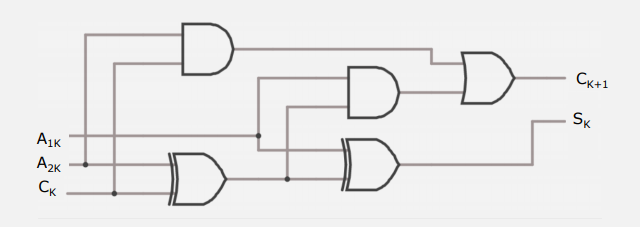
\includegraphics[scale=0.6]{IM_full_adder_bis}
  \caption{Most efficient way to create a full adder, by using two XOR gates, two AND gates and one OR gate}
  \label{FullAdderCircuit}
\end{figure}

\subsection{Ripple carry adder} \label{RCA_Section}

If we align a series of full adders we obtain a ripple carry adder (shortened in RCA).

\vspace{3mm}

This circuit is useful because it can perform not only sums among positive numbers, but also algebraic sums. We point out that in our circuit only the second addend could be negative.

\vspace{3mm}

This happens because, in our circuit, both numbers are considered positive, but the user can pick the subtraction operation, which makes the second addend negative. It is not possible to modify the sign of the first number.

\vspace{3mm}

In figure \ref{RCA_SMALL} you can see a ripple carry adder with a 3-bit input (where one of the bits if the sign bit).

\begin{figure}[h]
  \centering
  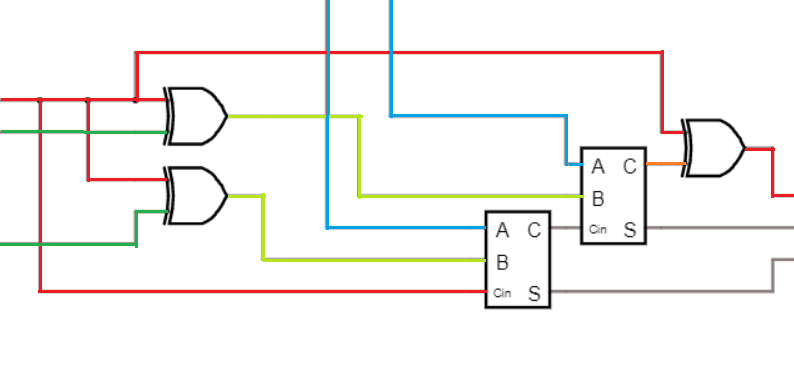
\includegraphics[scale=.65]{IM_RCA_SMALL.PNG}
  \caption{3-bit ripple carry adder}
  \label{RCA_SMALL}
\end{figure}

We can list its working steps:
\begin{enumerate}
  \item The digits of the first number (blue wires, one per digit) enter the full adders.
  \item The digits of the second number (green) get compared to the sign bit (red) by two XOR gates. They will exit these gates on the lime wire, and they will enter the full adders too. If the second number is negative, the red wire will be on, and the digits will be inverted, following the rule on how to obtain the opposite of a binary number.
  \item Considering that the opposite of a binary number is $-A=NOT(A)+1$, the "1" is added in the first full adder as a $C_{in}$.
  \item The sum is performed and the result goes to a decoder. The XOR gate on the right side of the image compares the sign bit with the carry-over of the last sum performed (orange). 
  
    \vspace{3mm}

    Let's consider the possible cases of this last XOR gate:
  \begin{enumerate}
    \item If the sign bit is 0 and the carry-over of the last full adder is 0, this means we are summing two positive numbers, which result is positive, as confirmed by the XOR.
    \item If the sign bit is 0 and the carry-over of the last full adder is 1, this means we are experiencing a memory overflow. The result goes beyond the range the calculator can handle.
    \item If the sign bit is 1 and the carry-over of the last full adder is 0, this means we are subtracting two numbers, and the second has a greater module. So the result is negative.
    \item If the sign bit is 1 and the carry-over of the last full adder is 1, this means we are subtracting two numbers, and the first has a greater module. So the result is positive.
  \end{enumerate}
\end{enumerate}

\section{Decoder} \label{DecoderSection}

The decoder is a device complementary to the encoder, as it ``translates'' a binary input into a more readable decimal output.

\begin{figure}[h]
  \centering
  %\captionsetup{justification=centering,margin=2cm}
  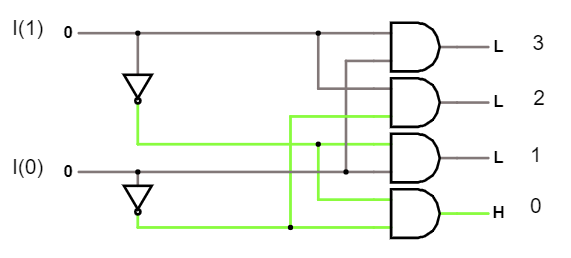
\includegraphics[scale=0.7]{basic_decoder}
  \caption{Here's a basic 2-bit decoder}
  \label{basic_decoder}
\end{figure}

Each output line is connected to an AND gate. Each AND is connected to every single input line, either directly or through an inverter. This way, the AND gate returns a high voltage only if the inputs match the binary representation of its corresponding output line.

\begin{table}[h]
  \centering
  \begin{tabular}{| c | c || c | c | c | c |}
  \hline
  I$_1$ & I$_0$ & O$_0$ & O$_1$ & O$_2$ & O$_3$ \\ \hline
  0 & 0 & 1 & 0 & 0 & 0 \\ \hline
  0 & 1 & 0 & 1 & 0 & 0 \\ \hline
  1 & 0 & 0 & 0 & 1 & 0 \\ \hline
  1 & 1 & 0 & 0 & 0 & 1 \\ \hline
  \end{tabular}
  \caption{Truth table for the 2-bit decoder}
  \label{Table_basic_decoder}
\end{table}

\clearpage

\section{Real calculator (3-bit)}

Now that the 3 key parts of a basic calculator have been introduced, we can try to assemble one in lab. This real calculator will be quite small and simple, for both time limitations and materials availability. 

\subsection{The blueprint}

\begin{figure}[h]
  \centering
  %\captionsetup{justification=centering,margin=2cm}
  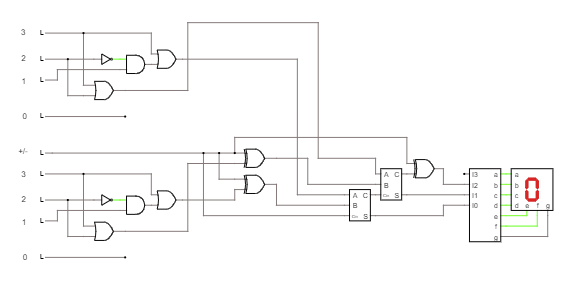
\includegraphics[scale=0.8]{real_calculator_blueprint}
  \caption{Here's the blueprint of our calculator}
  \label{real_calculator_blueprint}
\end{figure}

In Figure \ref{real_calculator_blueprint} is showcased the blueprint of our calculator. It receives 2 2-bit numbers as inputs, encodes them in binary and then adds them up using a 2-bit ripple carry adder. A decoder then converts the result in decimal and displays it.

\vspace{3mm}

There is also an additional input line useful to perform the subtraction. When this input line is low, the 3 XOR gates can be ignored as they return the unchanged input.

\vspace{3mm}

When the subtraction line is high, however, those gates return the opposite of said input lines. This is very important, as the first 2 XOR gates have the specific purpose of converting the second input into its opposite.
%MARCO E ALESSANDRO RITENGONO CHE QUESTA PARTE SULLA SOTTRAZIONE RIDONDI MOLTO. E' GIA' SPIEGATA NEL RIPPLE CARRY ADDER. MANTIENINE, SE PROPRIO PROPRIO, UNA VERSIONE MOLTO RIDOTTA, CHE COMUNQUE E' GRADEVOLE AL PALATO ^ω^ <-- Marco forced me to do this smile (questa parte, come quella sull'orologio del Riboldi, VA MANTENUTA ANCHE NELLA VERSIONE DEFINITIVA COME COMMENTO)

\vspace{3mm}

Effectively, when the subtraction line is high, we are adding two signed 3-bit numbers, a negative number and a positive number. To do that, we would need a 3-bit ripple carry adder, but:

\begin{itemize}
  \item The first input is always positive, so its sign bit its always 0 (in fact, it doesn't even exist). So, we only need an additional half-adder;
  \item We are not intrested in the carry bit of the last half-adder, as we are working with 3-bit numbers.
\end{itemize}

But a half-adder circuit without the carry output is a XOR gate. This is precisely the purpose of the third XOR gate. With this configuration, the subtraction line does 3 things:

\begin{itemize}
  \item It endodes the second input into its opposite;
  \item Works as the sign bit of the second input;
  \item It is directly connected into the $C_0$ input of the first full-adder to add 1 to the final result.
\end{itemize}

As for the decoder, both in our blueprint and in lab we are going to use a pre-made decoder. Assembling a decoder using AND gates would require a significant amount of time and resources which we do not have access to.

\subsection{Breadboard 1}

The calculator has been assembled using 3 different breadboards. The first breadboard handles the input part and the encoding process.

\vspace{3mm}

The input part is created using a ``keyboard'', which is a series of 6 switches built into a compact board. 
%keyboard o switch table?
\begin{figure}[h]
  \centering
  %\captionsetup{justification=centering,margin=2cm}
  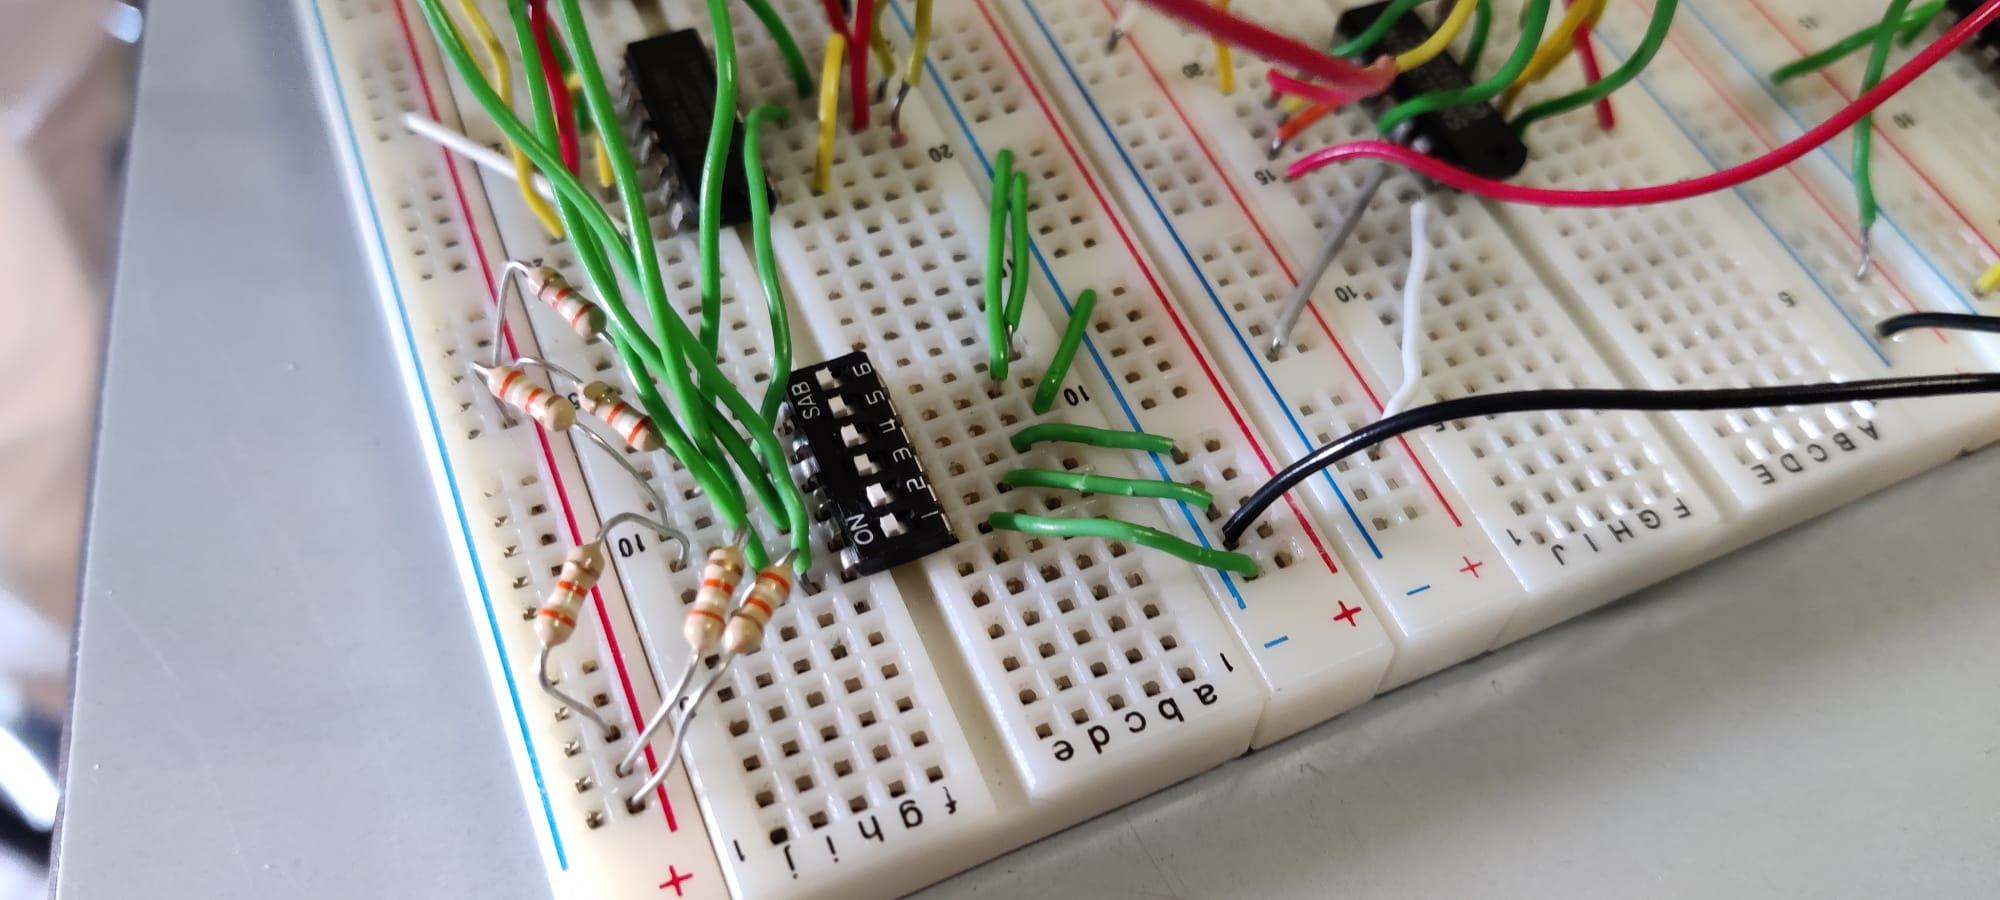
\includegraphics[width=\linewidth]{breadboard1_bis}
  \caption{The ``keyboard''}
  \label{breadboard1_bis}
\end{figure}

One side of each switch is grounded, while the other one is connected to the power supply through a resistor ($\approx 30-50 \; k \Omega$). 

\vspace{3mm}

When the switch is open, there is no current flow through the resistor and therefore no voltage difference across the resistor. Any high impedance input device can then be connected to the second end of the resistor to read a high voltage.

\vspace{3mm}

When the switch is closed, the current is free to flow through the resistor down to earth. The second end of the resistor is at the same voltage as the ground, and the input device reads a low voltage.

\vspace{3mm}

This device allows us to conveniently manipulate 6 different input lines. We are going to use the switches 1, 2 and 3 to write the first input, and the switches 4, 5 and 6 to write the second (4 being 1, 5 being 2 and 6 being 3). To write 0, the user just needs to leave all the switches open.

\vspace{3mm}

The rest of the first breadboard is dedicated to the encoding process. The process works exactly as described in section \ref{PriorityEncoderSection}, with the right part of the board dedicated to the encoding of the first input and the left part dedicated to the second.

\vspace{3mm}

We are not going into the details of the wiring. We will just mention that the white wires are used to connect the gates to the power supply, and the black and brown wires are used to connect the gates to earth.

\begin{figure}[h]
  \centering
  %\captionsetup{justification=centering,margin=2cm}
  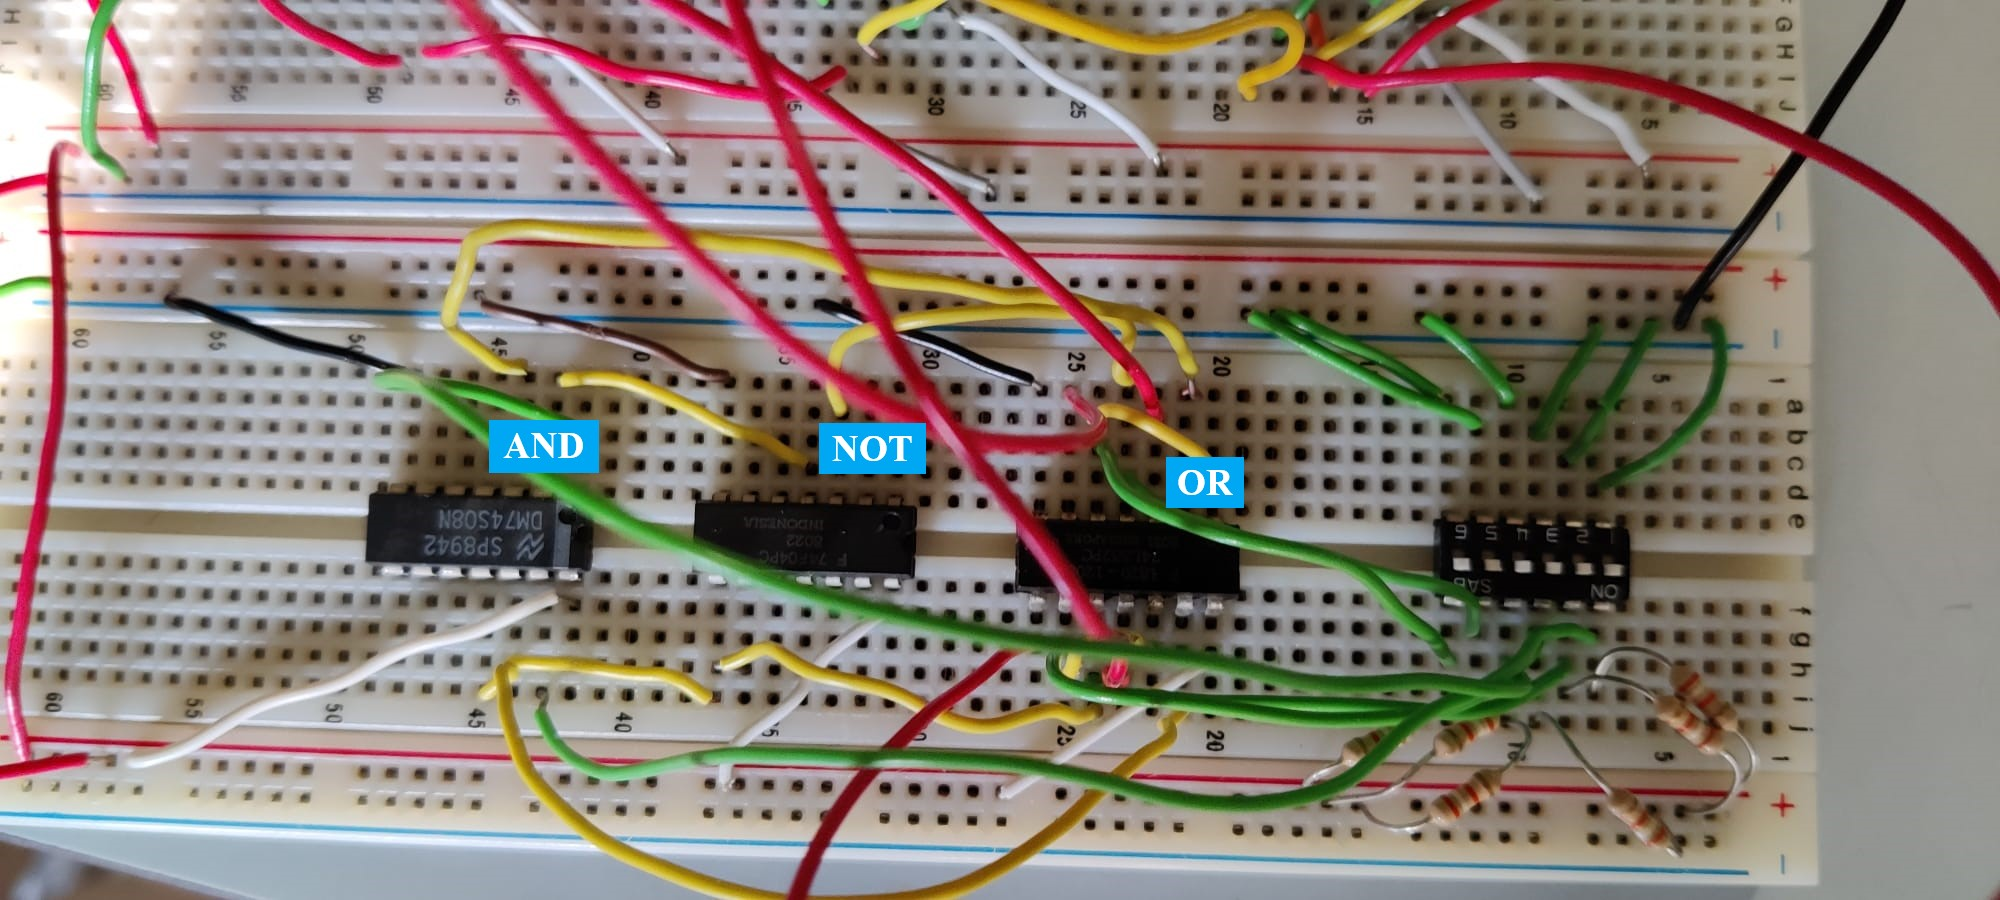
\includegraphics[width=\linewidth]{breadboard1}
  \caption{Breadboard 1}
  \label{breadboard1}
\end{figure}

\subsection{Breadboard 2}

The second breadboard handles the calculation process. It is a 2-bit ripple carry adder, composed of 2 full adders. The first full adder is on the left side of the board and the second adder is on the right side. The process works exactly as described in section \ref{RCA_Section}. 

\begin{figure}[h]
  \centering
  %\captionsetup{justification=centering,margin=2cm}
  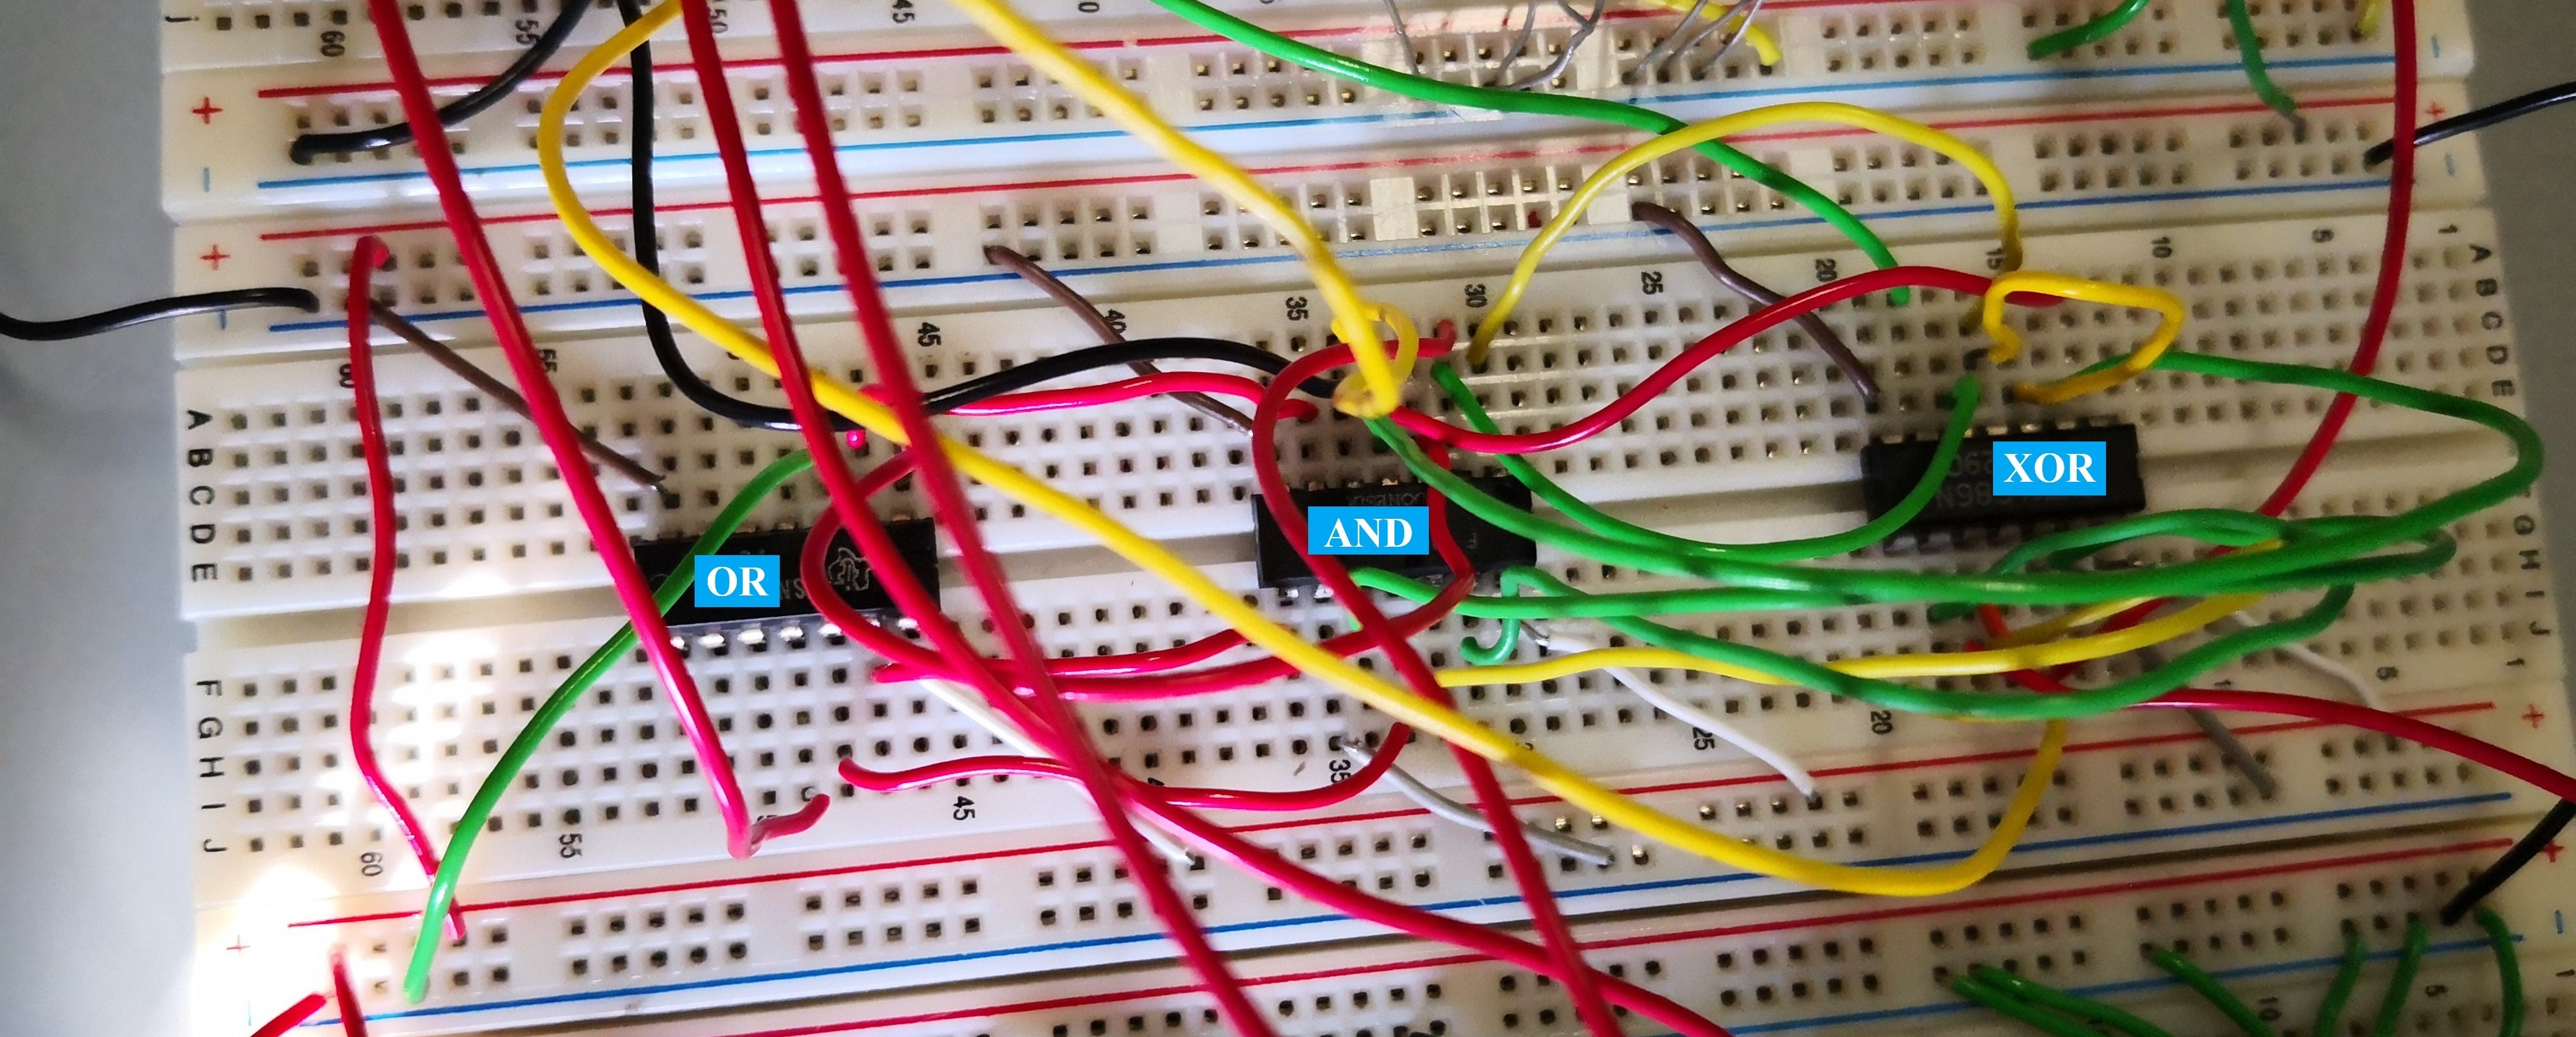
\includegraphics[width=\linewidth]{breadboard2}
  \caption{Breadboard 2}
  \label{breadboard2}
\end{figure}

\clearpage

\subsection{Breadboard 3}

The third breadboard handles the decoding process and houses everything that could not fit into the previous 2 breadboards. 

\begin{figure}[h]
  \centering
  %\captionsetup{justification=centering,margin=2cm}
  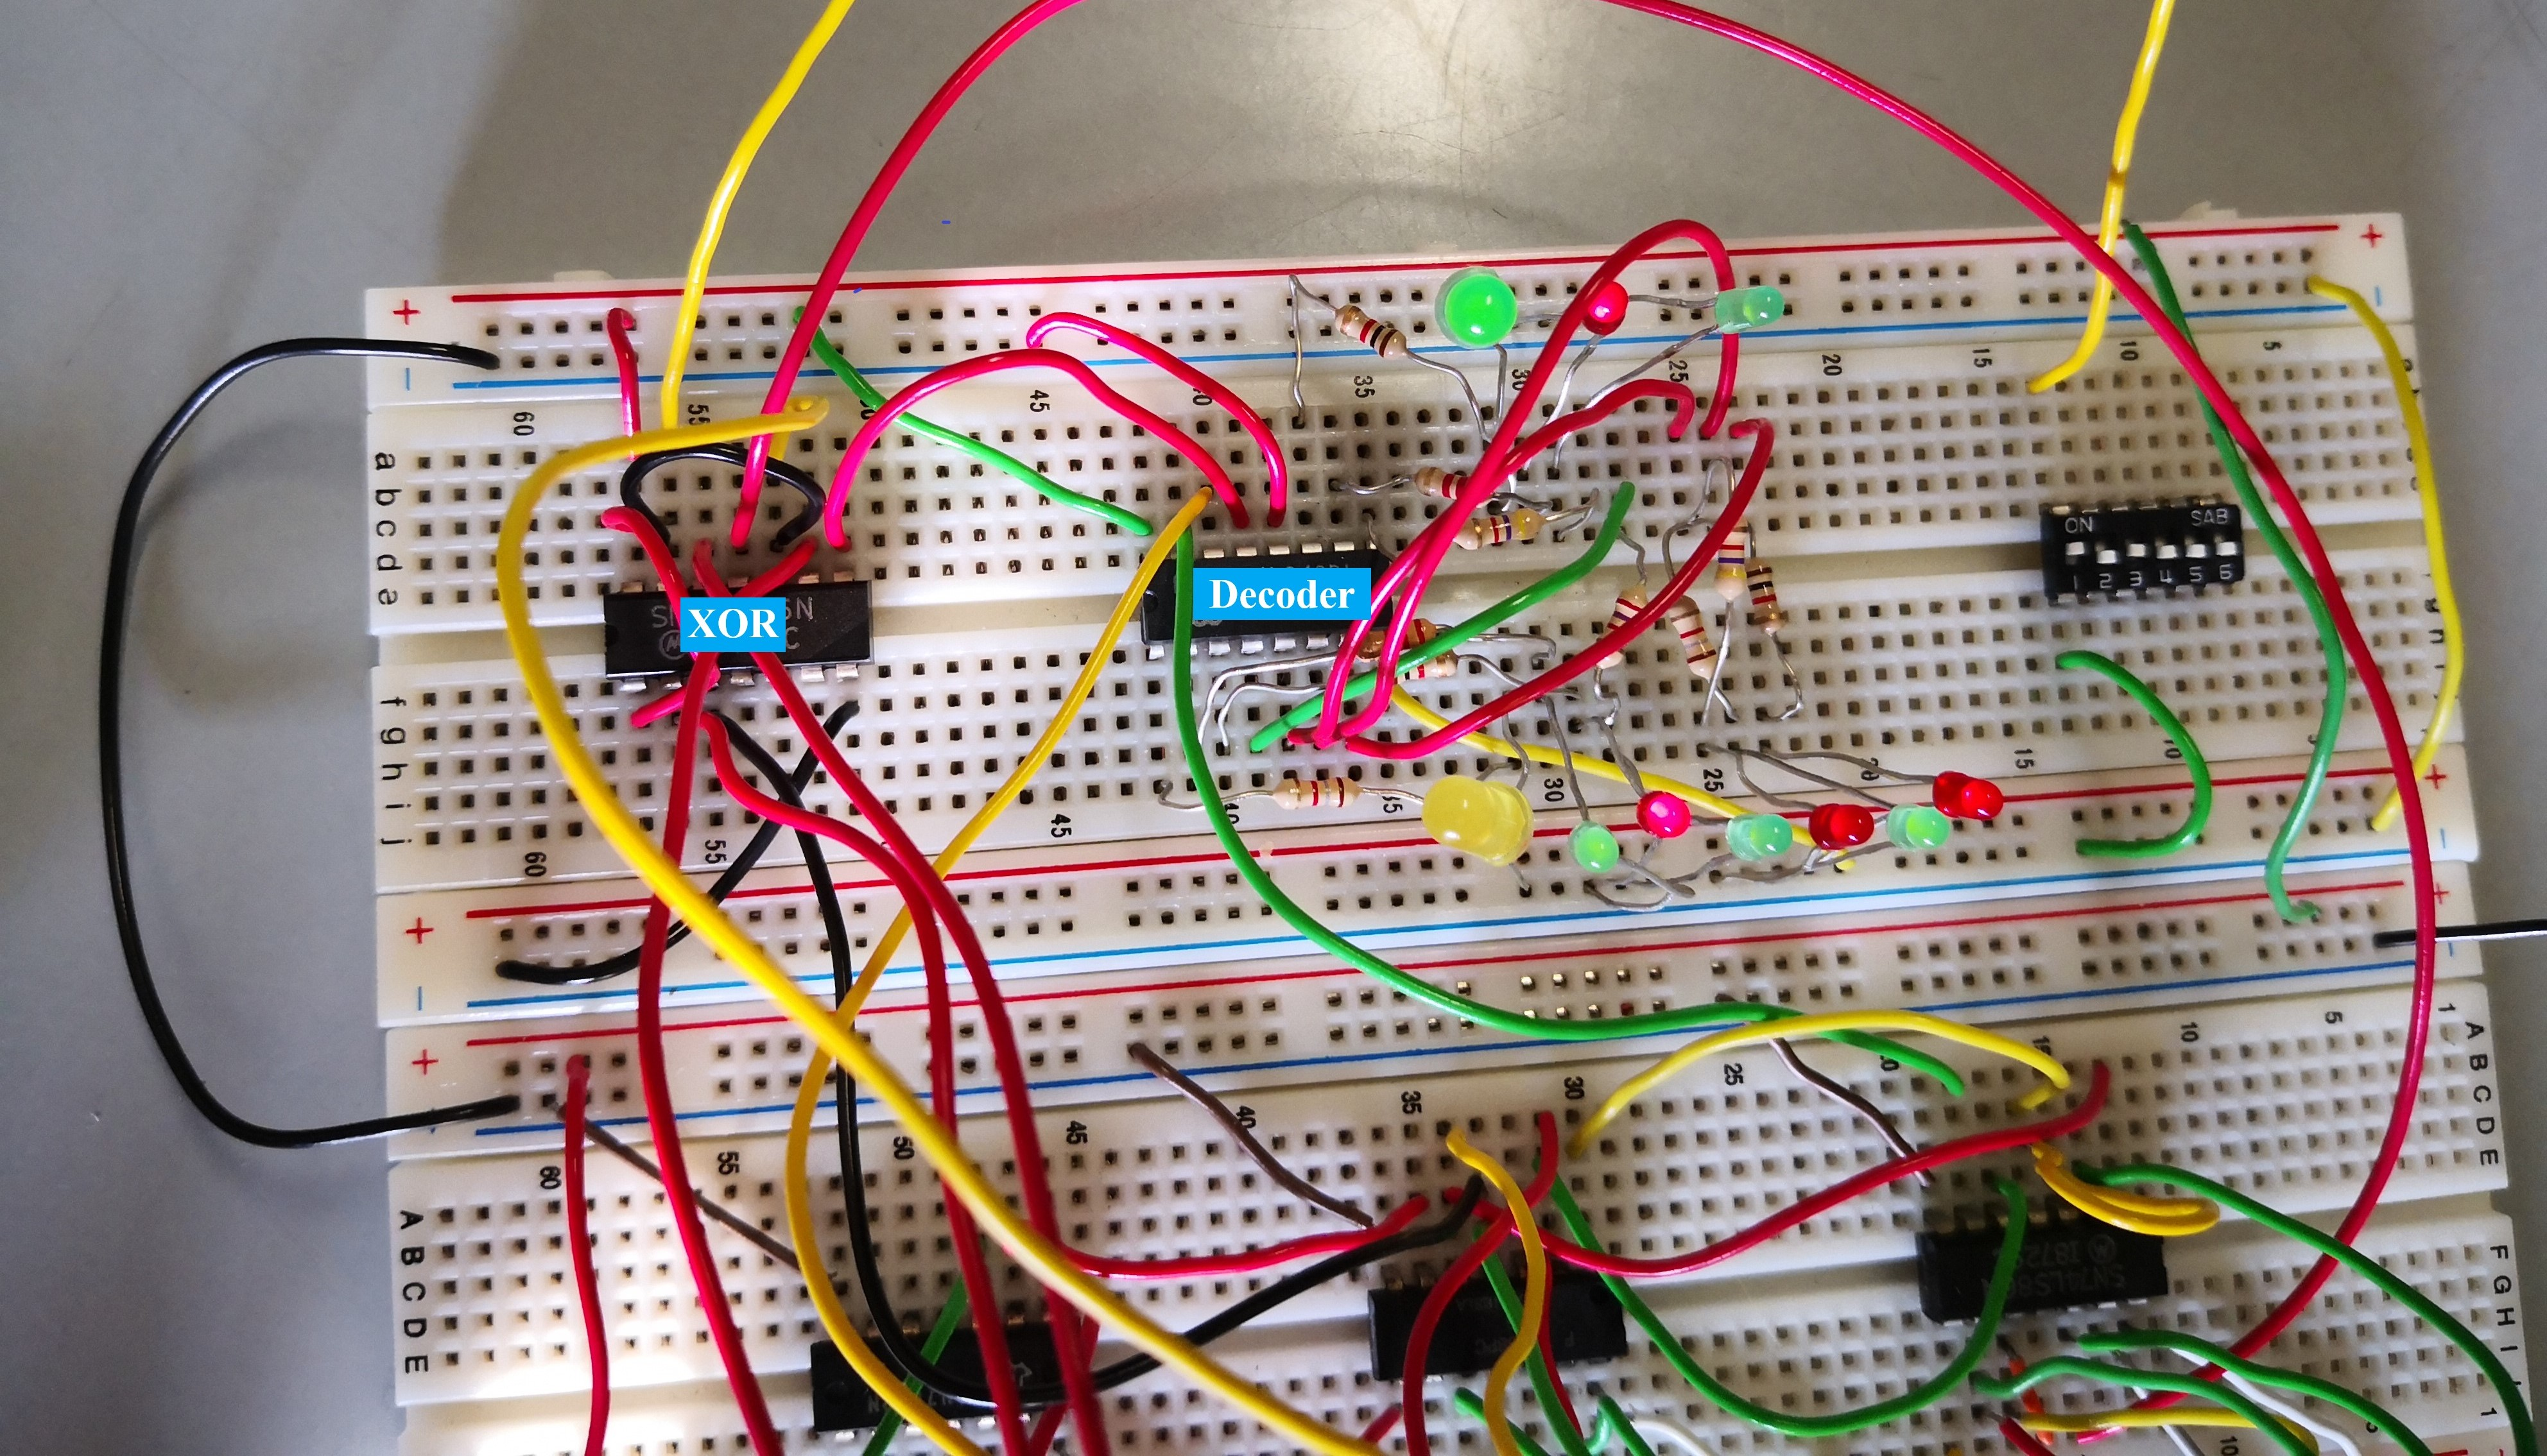
\includegraphics[width=\linewidth]{breadboard3}
  \caption{Breadboard 3}
  \label{breadboard3}
\end{figure}

The breadboard houses the 3 XOR gates necessary to enable the subtraction process. Those gates are connected to both the previous breadboards.

\vspace{3mm}

The decoder works in a similar way to what is described in section \ref{DecoderSection}. The only key difference is that it works using negative logic: a 1 output is low in voltage an a 0 output is high in voltage. 

\vspace{3mm}

To read our output more easily, we connected the 10 outputs to 10 LEDs. The decoded number corresponds to the least bright LED. The yellow LED corresponds to the number 0, and the value of the others can be deduced counting up going counterclockwise. The 8 and 9 LEDs are there for diagnostic purposes. Ideally, they should never turn off.

\vspace{3mm}

There is also a switch, whose purpose is to enable the operation of subtraction. While in our simulator the ``subtraction line'', and everything connected to it, was at low voltage when not connected to any power supply, in reality an isolated subtraction line finds itself at high voltage. 

\vspace{3mm}

To enable the addition/subtraction selection, then, we connected this line to earth through a switch. When the switch is open, the subtraction line is at ground potential and the calculator does the addition process. When the switch is closed, the subtraction line is isolated (high voltage) and the calculator does the subtraction process.

\clearpage

\subsection{The complete project}

\begin{figure}[h]
  \centering
  %\captionsetup{justification=centering,margin=2cm}
  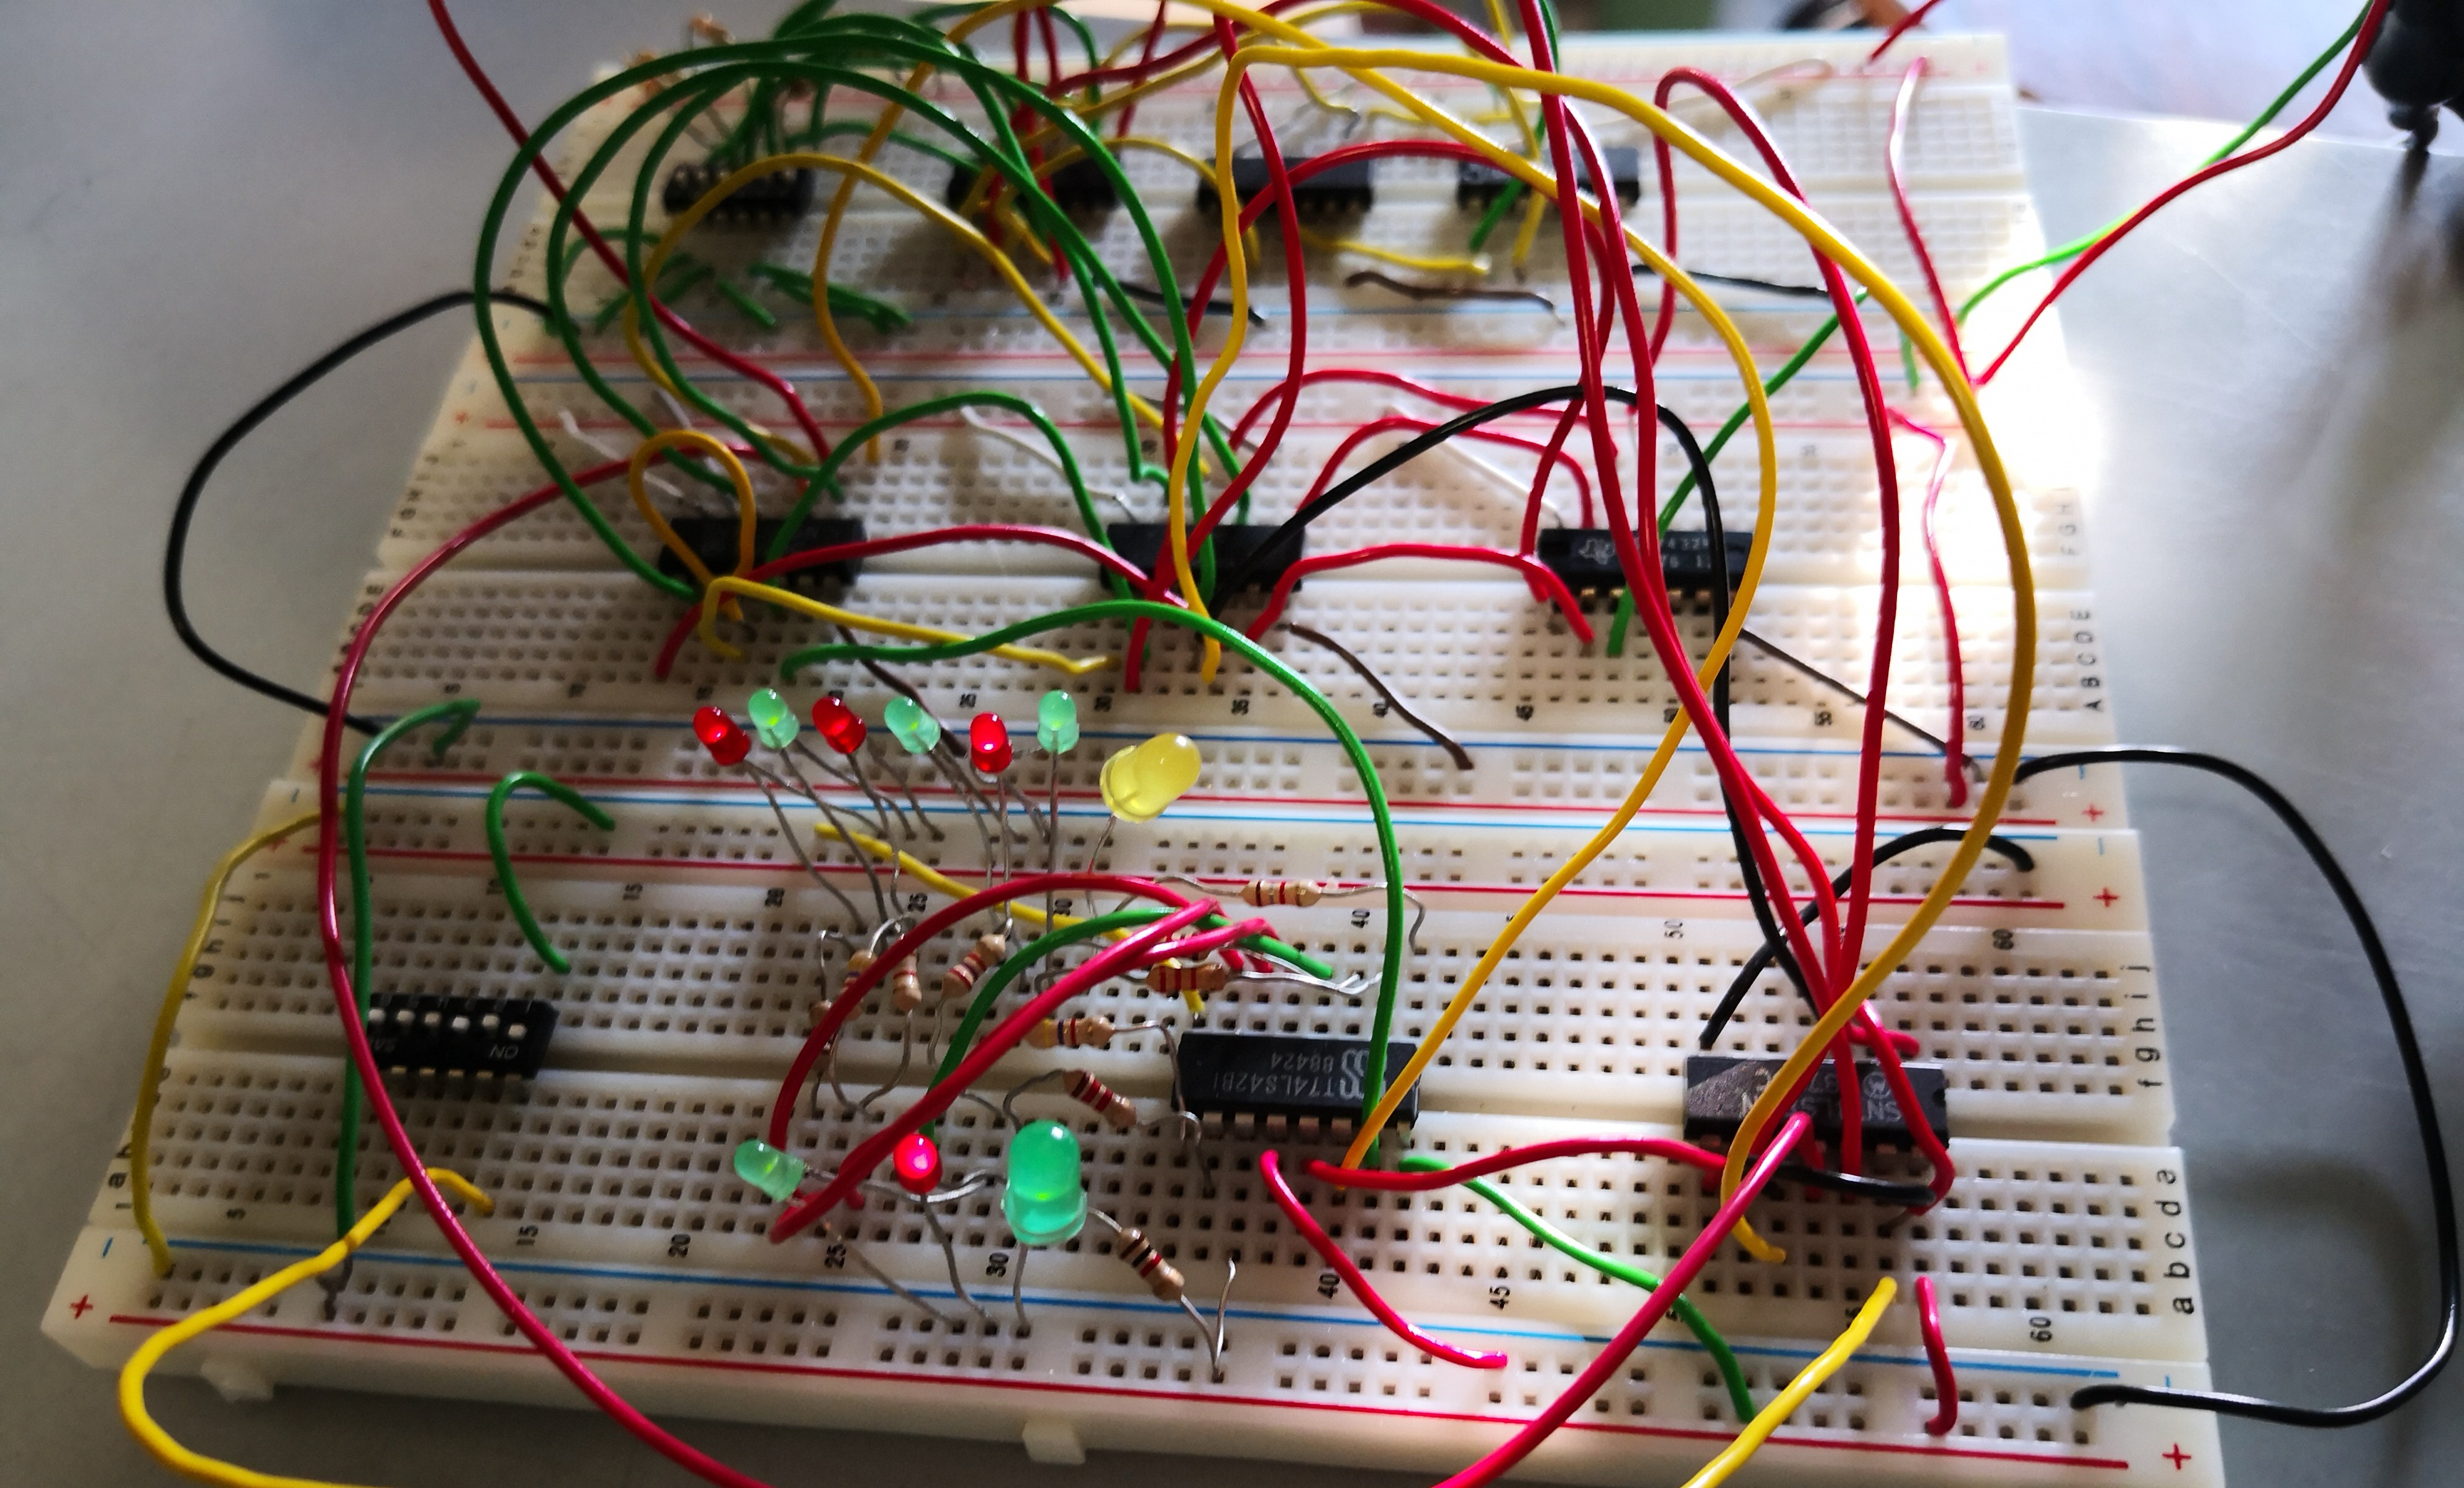
\includegraphics[width=\linewidth]{calculator}
  \caption{The complete 3-bit calculator}
  \label{calculator}
\end{figure}

After assembling the circuit, we then verified its truth table (Table \ref{Table_calculator}).

\begin{table}[h]
  \centering
  \begin{tabular}{| c | c | c | c ||| c | c | c | c ||| c | c | c | c ||| c | c | c | c |}
  \hline
  I$_A$ & I$_B$ & sub & O & I$_A$ & I$_B$ & sub & O & I$_A$ & I$_B$ & sub & O & I$_A$ & I$_B$ & sub & O \\ \hline
  0 & 0 & 0 & 0 & 0 & 2 & 0 & 2 & 0 & 0 & 1 & 0 & 0 & 2 & 1 & 6 \\ \hline
  1 & 0 & 0 & 1 & 1 & 2 & 0 & 3 & 1 & 0 & 1 & 1 & 1 & 2 & 1 & 7 \\ \hline
  2 & 0 & 0 & 2 & 2 & 2 & 0 & 4 & 2 & 0 & 1 & 2 & 2 & 2 & 1 & 0 \\ \hline
  3 & 0 & 0 & 3 & 3 & 2 & 0 & 5 & 3 & 0 & 1 & 3 & 3 & 2 & 1 & 1 \\ \hline
  0 & 1 & 0 & 1 & 0 & 3 & 0 & 3 & 0 & 1 & 1 & 7 & 0 & 3 & 1 & 5 \\ \hline
  1 & 1 & 0 & 2 & 1 & 3 & 0 & 4 & 1 & 1 & 1 & 0 & 1 & 3 & 1 & 6 \\ \hline
  2 & 1 & 0 & 3 & 2 & 3 & 0 & 5 & 2 & 1 & 1 & 1 & 2 & 3 & 1 & 7 \\ \hline
  3 & 1 & 0 & 4 & 3 & 3 & 0 & 6 & 3 & 1 & 1 & 2 & 3 & 3 & 1 & 0 \\ \hline
  \end{tabular}
  \caption{Truth table for the 3-bit calculator, where sub$=$0 means addition and sub$=$1 means subtraction}
  \label{Table_calculator}
\end{table}

Given that, in a 3-bit signed configuration, $7=-1$, $6=-2$, $5=-3$ and $4=-4$, we can conclude that our calculator works as intended.

\clearpage





\clearpage

\section{16-bit calculator} \label{SimulatedCalculator}



\subsection{Input with 16-bit}

Our goal is to create a 16-bit calculator. It has to receive 16 bits as input and that produces 17 output bits (the 17th is the sign bit).

\vspace{3mm}

One of the problems that arise when we want to use such a big memory space is the increasement in complexity; this makes the circuit more expensive and also takes a lot of physical space, that could be used for other purposes. In a small scale, we could use a 2-bit priority encoder, but, for our project, it would be unpractical and unnecessarily harder.

\vspace{3mm}

Another problem regarding the priority encoder, is that this component would require more physical space. We would need an input line for every single number we could insert. Considering that the possible inputs are all the natural numbers in the interval $[0,2^{16})$, we would need $2^{16}$ input lines.

\vspace{3mm}

To solve both problems we decided to use a keyboard. It takes the input through some buttons, instead of the levers we used in the laboratory. This method solved both the problem with the number of inputs and the problem of the complexity of the decoder.



\subsection{Keyboard}

The keyboard part connects a point at high voltage to the rest of the circuits. It is composed by: 

\begin{itemize}
    \item 10 buttons for the digits from 0 to 9;
    \item An addition button labeled $+$;
    \item A subtraction button labeled $-$;
    \item A button to have the result displayed, labeled $=$;
    \item A clear button that resets the entire circuit.
\end{itemize}

\begin{figure}[h]
    \centering
    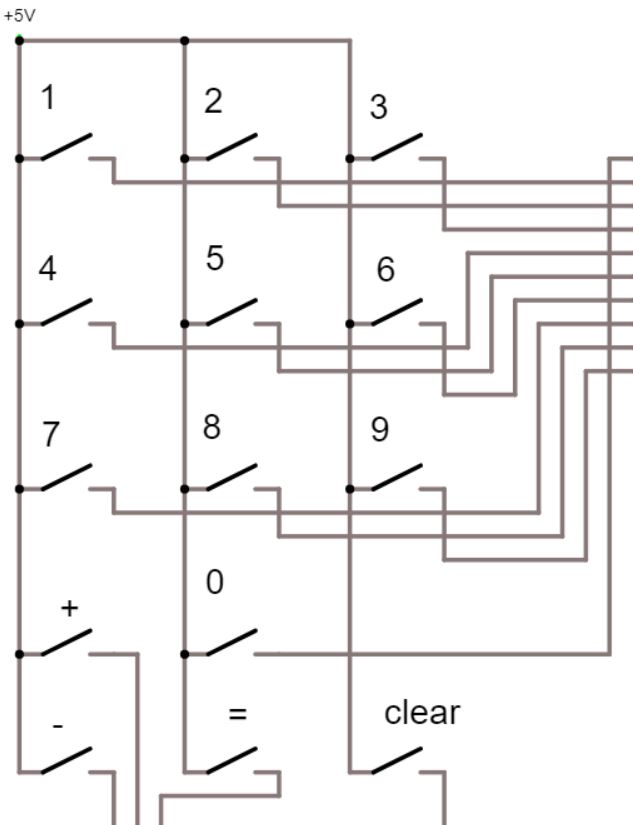
\includegraphics[scale=.3]{IM_Keyboard}
    \caption{Picture of the simulated circuited keyboard}
    \label{Keybaord}
\end{figure}

\clearpage

\subsection{4-bit encoder}
The first part of our encoder is a 4-bit encoder, without priority. 

\begin{figure}[h]
    \centering
    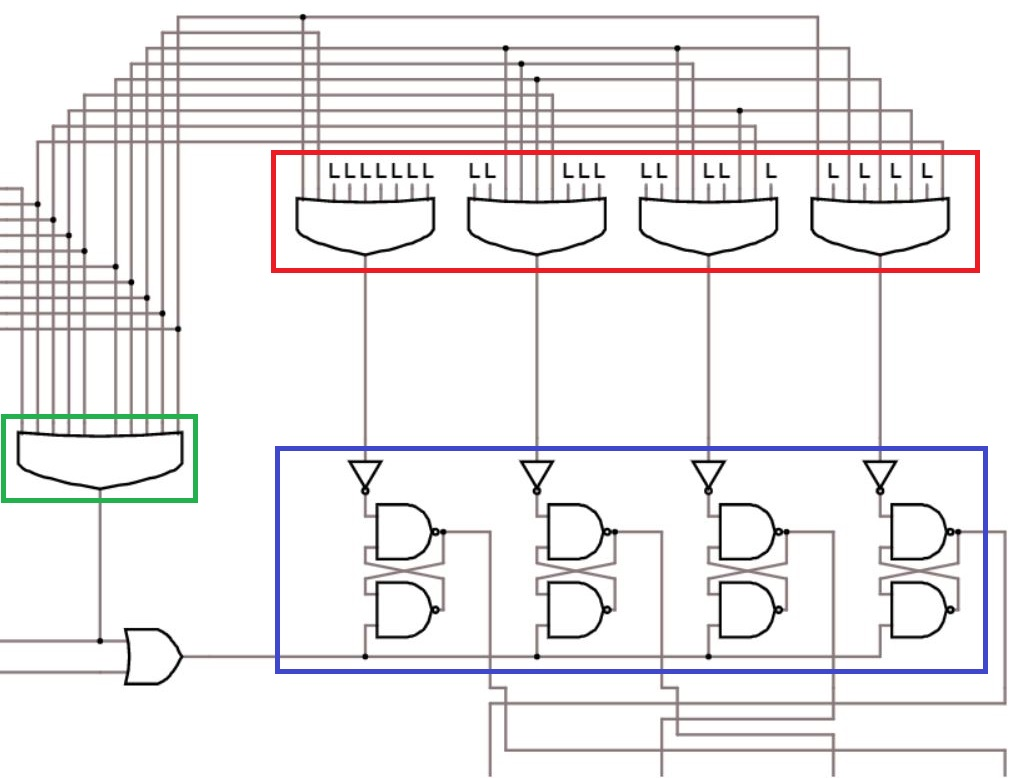
\includegraphics[scale=.35]{IM_4BitEncoder.JPG}
    \caption{4-bit encoder}
    \label{encoder}
\end{figure}

As you can see in figure \ref{encoder} this part can be split in three different sections:

\begin{itemize}
    \item The red part is a 4-bit encoder without priority. As we were saying in the paragraph above, the advantage of using a keyboard is that we will, under normal condition, only get 1 input at a time making a priority encoder useless. The encoder works by checking, with an OR gate, which bits the inserted number activates.
    
    \vspace{1mm}

    For example, if we press the button "6" the binary input will be $0110$, so only the second and the third bit will be activated.

    \item The green part is an OR gate connected to all the input lines, in order to check whether a button corresponding to a number is pressed. This choice has been made because if 0 was pressed, it would not result in any binary input, but it would be needed to multiply the previous number by $10$. 

    \item The blue part is a small "flash memory", which gets cleared when the input button is no longer pressed. 
            
        This part, whose functioning relies on the concept of bistable circuit, is a simple "security" method, useful to ensure that the inputs arrive correctly to the next memory. This part could be removed if the circuit timing was perfect, but we preferred to keep it to ensure no problem would arise.    
\end{itemize}


\subsection{Memory and successive inputs}

This part allows the circuit to receive consecutive inputs, and it is composed by two memories and two ripple carry adders. 

\vspace{3mm}

In this section the input gets stored and, after a new button is pressed, the stored number is multiplied by 10 and then added to the new input. By doing this we can obtain every number within the memory limit.
\clearpage
It is important to point out that this part works by using the concepts of "rising edge", where the input passes from a low state to a high one, and "falling edge", where the input changes from high to low. This concept makes possible to process a single input in two phases.

\begin{figure}[h]
    \centering
    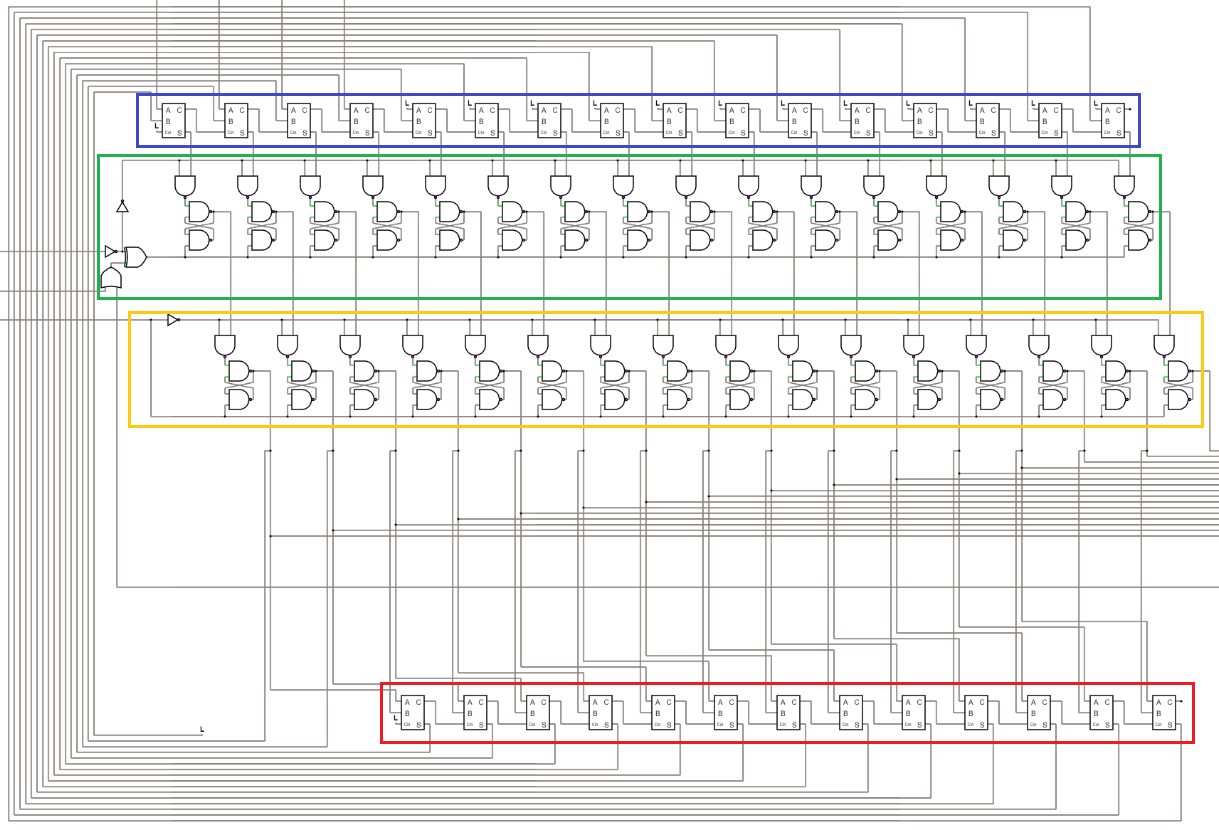
\includegraphics[scale=.55]{IM_Converter.PNG}
    \caption{The two memories (green and yellow), the 10x multiplier (the red RCA) and the adder (the blue RCA)}
    \label{Converter}
\end{figure}


\subsubsection{Rising edge}

When the first button is pressed, the circuit is in a state of "rising edge". In this moment, the horizontal wire that goes to all the NANDs of the second memory (highlighted in yellow in figure \ref{Converter}), switches to low to prevent the NANDs from letting any signal pass from the first to the second memory.

\vspace{3mm}

The second wire involved is the horizontal one under the first memory (highlighted in green), that also turns off. This wire is responsible for clearing the memory. This happens when this wire switches from high to low.

\vspace{3mm}

After a little while, the last wire that changes its state is the one on top of the first memory. This allows a new input to be memorized in the cleared memory.

\vspace{3mm}

It is important to note that, during the data storage, the reset wire (the horizontal one at the bottom of the green box) is in a low state, since it cleared the memory right before the storage of new data.

\vspace{3mm}

This last fact does not cause any trouble when the input is 0, since we are in the case 5 or 6 of the flip-flop truth table (table \ref{FlipFlopTT}) and, as you can see, the output is 0. 

\vspace{3mm}

The problem arises when the input data is 1, since we are in case 1 or 2 of the flip-flop truth table, where the two inputs are 0. As we can see in the truth table, in this case, both outputs are set at 1.

\vspace{3mm}

After one of the two inputs switches from low to high, the flip-flop returns in a normal state (state 3-6). But, to store a bit "1", we need to go from states 1 or 2, to state 4 of the truth table. In other words, as long as the clear line is the first one switching from low to high, we easily pass from state 1-2 to state 4.

\vspace{3mm}

Note that, it is not possible to reach state 3 in the case explained before, because state 1-2 "NewQ" becomes state 4 "OldQ" while state 3 "OldQ" is 0.

\vspace{3mm}

The problem we have just described has been solved in the simulated calculator by using the delay given from the logic gates. In reality, this could be a problem since this relies on physical properties that could depend from temperature, making this kind of timing, whether applied to a real circuit, not as precise as in the simulator.

\vspace{3mm}

The timing problem also includes the fact that the operation on the second memory should be done before the one on the first memory. In our circuit, this delay is performed by the "clearing part" (the XOR gate on bottom left corner of the green box). 

\vspace{3mm}

Another possible solution could be using an external clock to define when the action should be performed. But, in order to keep our simulated circuit as easy as possible, we decided to simply address the problem in this report.




\subsubsection{Falling edge}

After the the number button is released the circuit is in the "falling edge" phase.

\vspace{3mm}

The process is similar to the previous one. The first wire to change its state is the horizontal one below the second memory, this time. Its task is the memory reset, like the one in the first memory. After this, the horizontal wire on top of the second memory changes its state, to allow the second memory to store information coming from the first.

\vspace{3mm}

The last connection that switches is, as before, the horizontal one on top of the first memory. It switches from high to low and prevents any further memory modification.

\vspace{3mm}

The problem described at the end of the rising edge is, in fact, a problem that begins with the rising edge and ends during the falling edge. Since the first memory works during the rising edge phase, and the second one works during the falling edge phase, the second memory will suffer the same problem, and so it will have the same possible solutions explained before.


\subsubsection{Ripple carry adders}

This circuit works with two ripple carry adders.

\vspace{3mm}

During a calculation, the RCAs do not work at the same time. The first RCA, highlighted in blue lets the inserted digit head towards the first memory highlighted in green. Then, this digit passes through the second memory (yellow), during the falling edge phase, and gets multiplied by 10 from the red RCA. This multiplied digit is not used unless a new digit is inserted by the user.

\vspace{3mm}

If a new number button is pressed, this new value gets summed to the previous data, already multiplied by 10, and stored in the green memory. The sum of the two number is performed by the blue RCA.

\vspace{3mm}

If a third digit is inserted, the process repeats again.

\vspace{3mm}

Moreover, we can notice that after multipling by 10, the first bit is always set to 0. The second and the third bits depend only from the first and second bit of the original number, because they are only affected by the multiplication by 2 (0010) and not by the multiplication by 8 (1000). 

From the fourth bit the addition performed by the red RCA is needed because these binary digits are influnced by the 10x multiplication. %rivedere sta parte perchè ci sto capendo poco io che la sto scrivendo, che cazzo






\subsection{Sign bit}

To do the subtraction we could have used the full subtractor, but we decided to use the addition between positive and negative numbers in binary. To perform the subtraction we needed a way to read whether the second number was positive or negative . As visible in figure \ref{SignBit} we simply used a flip-flop. From the top (coming from the left side):
\begin{itemize}
    \item The first horizontal line is the input $+$;
    \item The second is $-$;
    \item The third is the clear signal, that also resets the sign bit.
\end{itemize}

\begin{figure}[h]
    \centering
    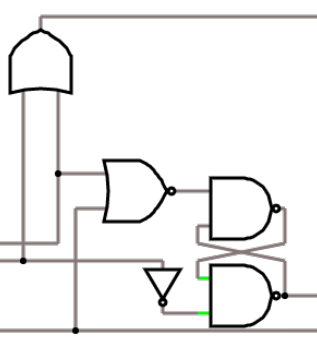
\includegraphics[scale=.5]{IM_SignBit}
    \caption{The component used to check a number sign, created with a flip-flop}
    \label{SignBit}
\end{figure}

\clearpage
\subsection{Memory}
The final part of the input is composed by the two memories in figure \ref{Memories}.

\begin{figure}[h]
    \centering  
    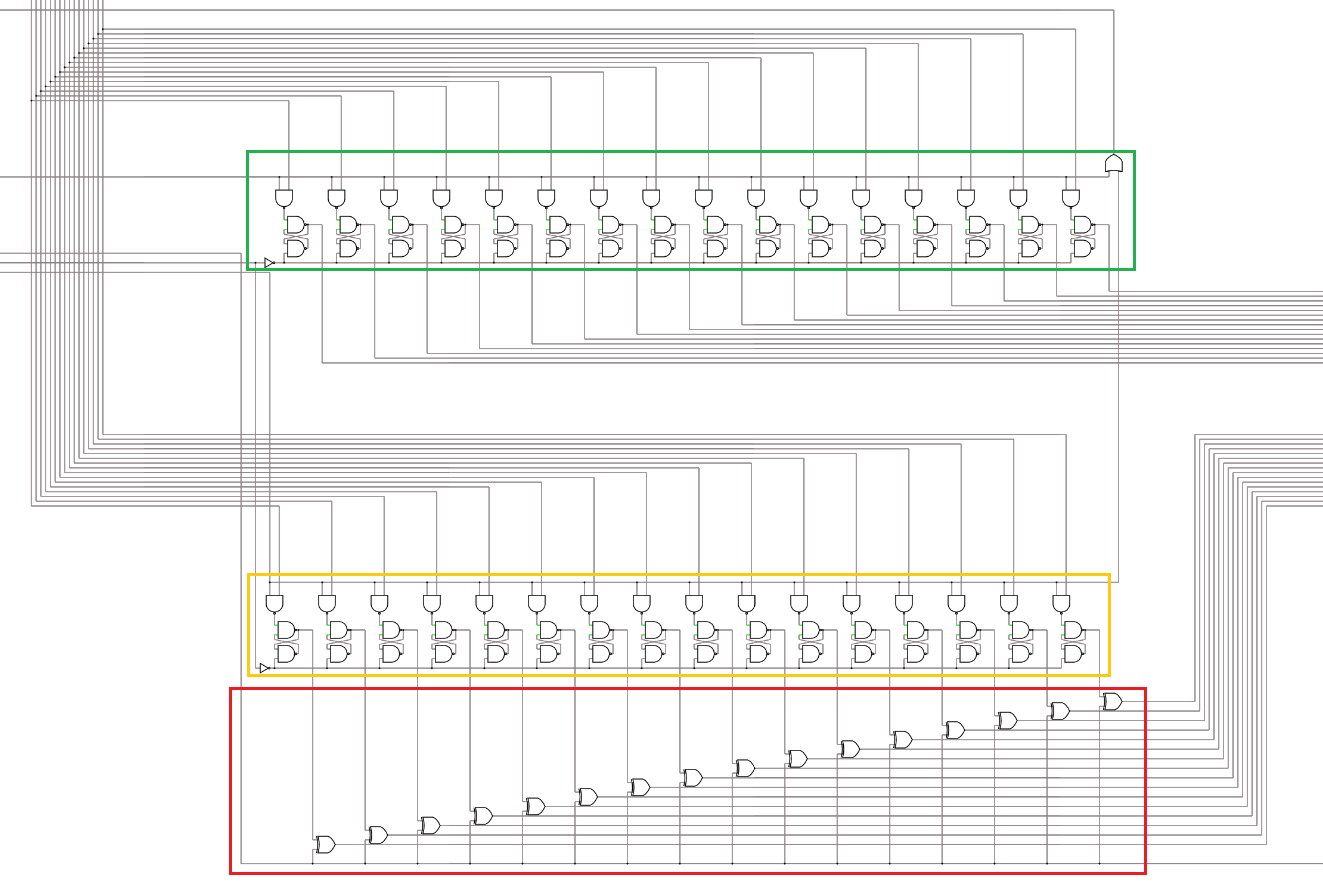
\includegraphics[scale=.5]{IM_Memories.PNG}
    \caption{Final part of the input section, composed of two memories, one for each number that needs storage}
    \label{Memories}
\end{figure}

\vspace{3mm}

The first memory, highlighted in green, is where the first number gets stored. Considering that, the first number is always positive, we can save it and give it to the processing section, just as it is. 

\vspace{3mm}

Since we want this memory to be modified only when it has to register the first number, we added the "NAND wire" that is the wire exiting the OR in figure \ref{SignBit}. This horizontal wire is located over the green memory.

\vspace{3mm}

With this, the memory will store information only when $+$ or $-$ are pressed. The vertical wire that exists the OR gate on the top right corner of the green memory is responsible of clearing the green memory in figure \ref{Converter}, making it possible to insert the second number.

\vspace{3mm}

The second memory, highlighted in yellow, works in the same way as the first one, but it stores the number when the "=" button in pressed.

\vspace{3mm}

The XOR gates beyond the yellow memory invert the bits of second number, as already explained in section \ref{RCA_Section}, when the user is doing a subtraction.

\subsection{Clear}

The last input, not discussed yet, is the clear button. This button is connected to the reset line of all the memories and the sign bit, and it switches every flip-flop to 0. 

\subsection{Processing}

The processing phase of the 16-bit calculator is done as explained in section \ref{RCA_Section}.

\begin{figure}[h]
  \centering
  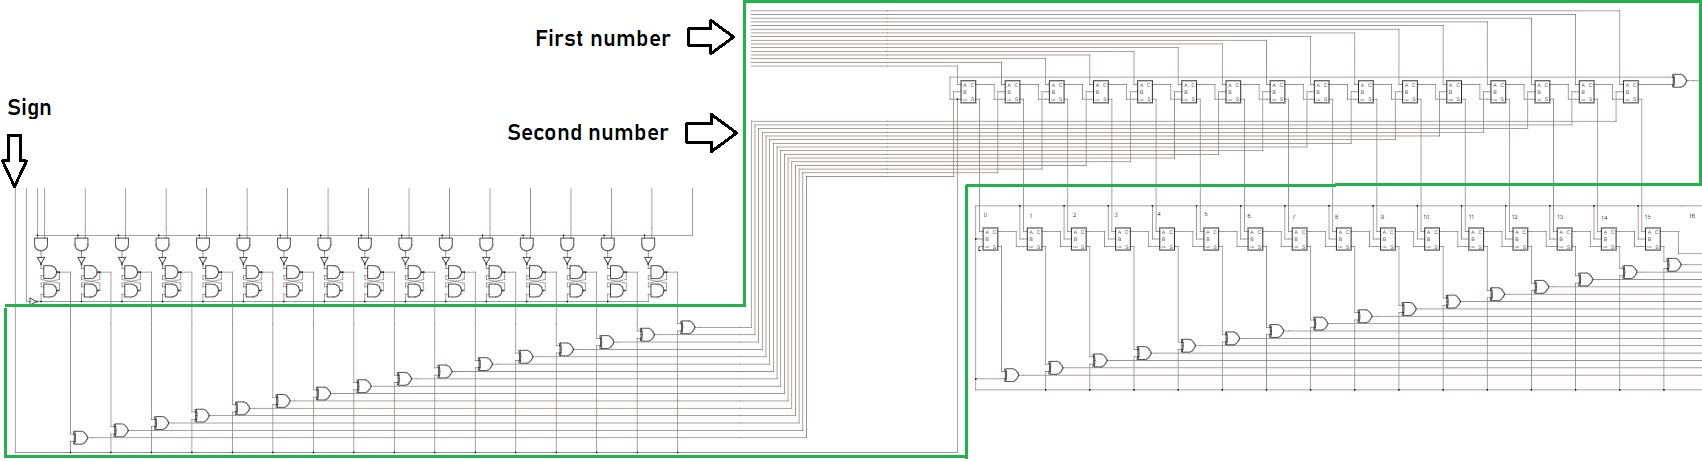
\includegraphics[scale=.4]{SC_Processing_Total.JPG}
  \caption{Processing section of the 16-bit calculator. The XOR gates in the bottom left zone are the ones highlighted in red in figure \ref{Memories} }
  \label{ProcessingTotal}
\end{figure}

\begin{figure}[h]
  \centering
  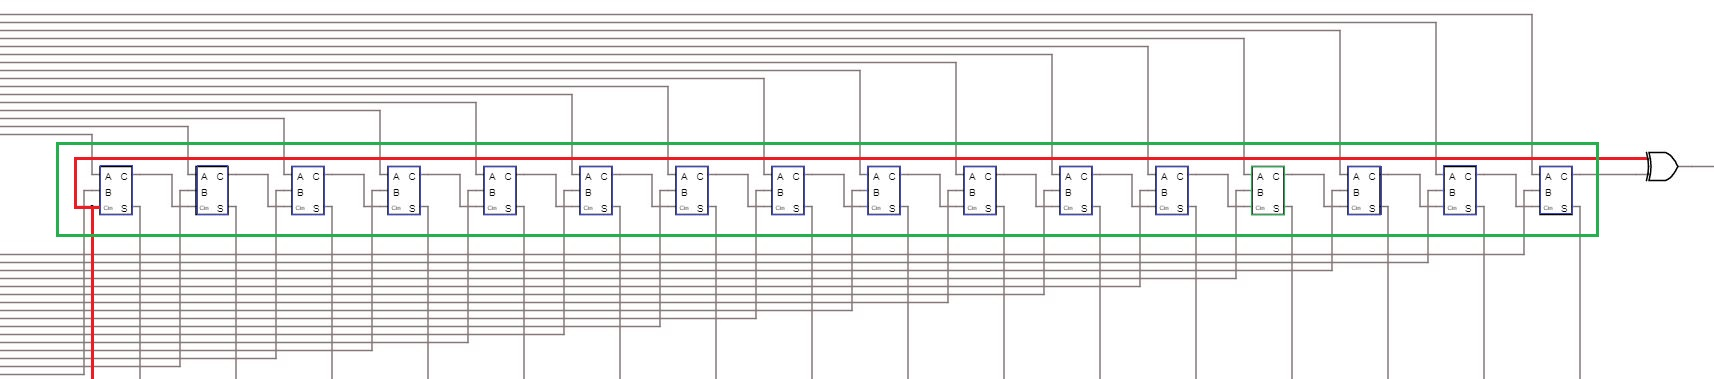
\includegraphics[scale=.4]{SC_Processing2.JPG}
  \caption{Ripple carry adder to sum the first and the second number. The red wire is the sign bit}
  \label{Processing2}
\end{figure}

The results that exit the RCA will go to the decoding part.




\subsection{Decoder}

After the inputs have been processed, it is needed a decoder (see figure \ref{Decoder}) in order to convert the output from binary to its decimal form.

\vspace{3mm}

The theorical largest number, in absolute value, that can be outputted by 17 bits (one of them is the sign bit) is $2^{16}$. So the decoding circuit needs to have 5 led displays for the digits and one extra display for the sign. It is possible to note that the image shows a 6th led display for the digits, because we originally thought, by mistake, we could have a 18 bit output.

\vspace{3mm}

We decided to operate the binary-decimal conversion with the so called "double dabble" circuit, that will be explained later in the report. Nevertheless this was not the main problem. The double-dabble converts positive numbers perfectly, but not negative ones. So we had to convert a negative number, if outputted, to a positive one and send the sign to the sign led display.

\begin{figure}[h]
    \centering
    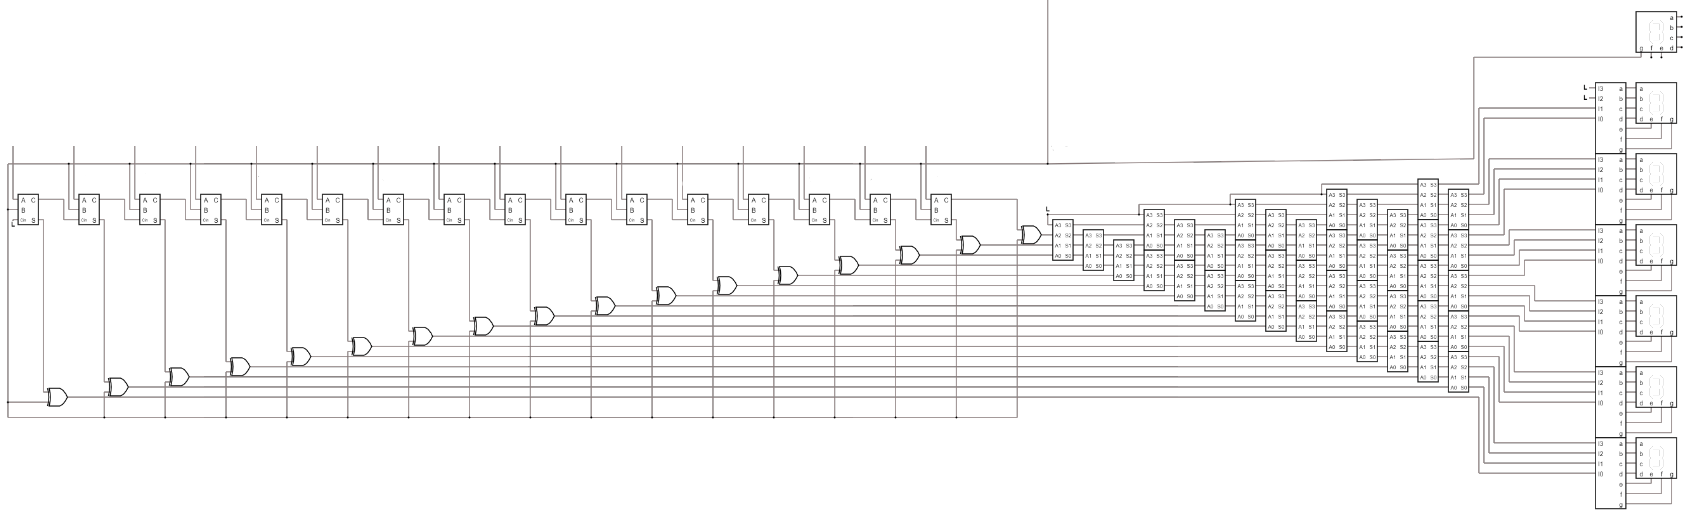
\includegraphics[scale=0.42]{SC_Decoder}
    \caption{Picture of the decoder}
    \label{Decoder}
  \end{figure}

\subsubsection{About the number sign}

The number sign has to be taken into account before converting the number into its decimal form. The number is a 16-bit binary, as already said, and it has one extra bit for the sign.

\vspace{3mm}

This part of the circuit (represented in figure \ref{Converter_bis}) uses a ripple carry adder and XOR logic gates, components that got already discussed in the previous sections. After the operation has been done between the two inputs, the first 16 bits reach the A input the full adders (the green lines in figure \ref{Converter_bis}), whereas the sign bit follows the red path.

\vspace{3mm}

This sign bit reaches every full adder B input, and also the XOR gates, that compare the result of the single full adders with the sign bit. The sign bit is true (or 1) when the number is negative and 0 otherwise. This allows the full adders to sum 1, following the formula above, if the processing output is negative, whereas if it is positive the number just stays the same.

\vspace{3mm} 

After this, the XOR gates, which truth table is give the final result, which will go to the double dabble.

\begin{figure}[h]
    \centering
    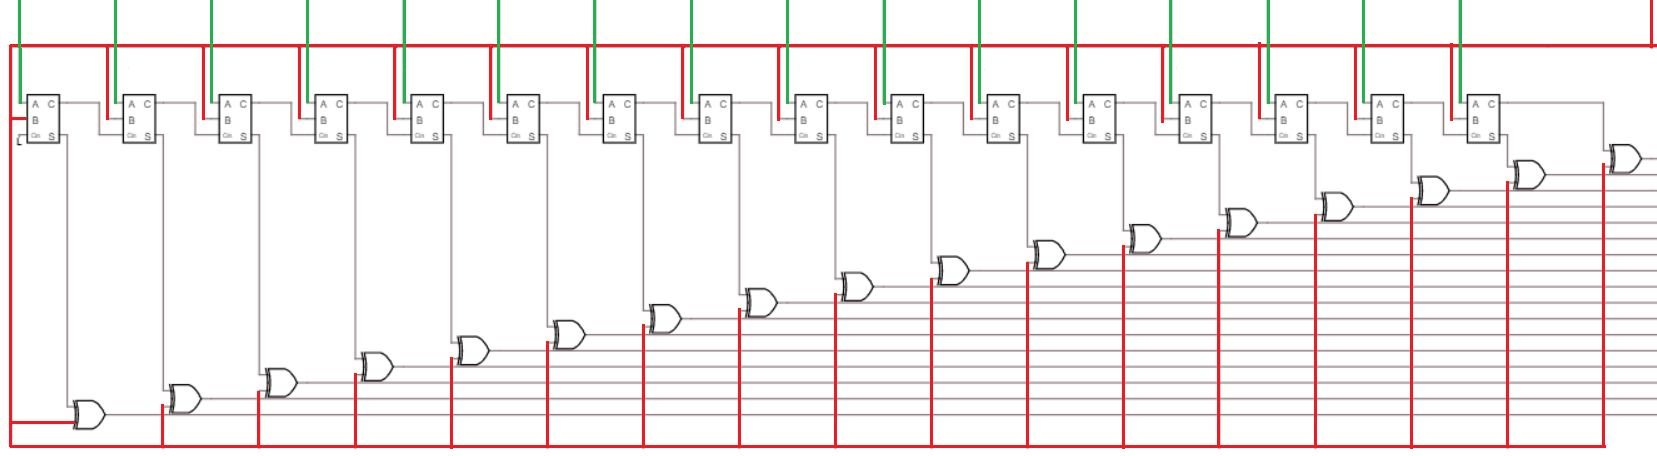
\includegraphics[scale=0.43]{SC_Converter.PNG}
    \caption{Picture of the first part of the decoder}
    \label{Converter_bis}
  \end{figure}
\pagebreak
\subsubsection{Double dabble}

This second part of the decoder is reached by the number that needs to be converted into decimal form. 

\vspace{3mm}

The entire circuit relies on an algorithmic process, based on the concept of "shift and add 3", which is the name of the component that mostly populates figure \ref{DoubleDabble}.

\vspace{3mm}

This algorithm takes a binary number and after having processed it gives an output divided into smaller parts composed of 4 bits each. Everyone of these parts will be then elaborated by 7 segment decoders and represent a single digit of the decimal number. The 7-segment decoders are obviously connected to 7-segments led displays, that can be seen on the right side of figure \ref{DoubleDabble}.

\begin{figure}[h]
    \centering
    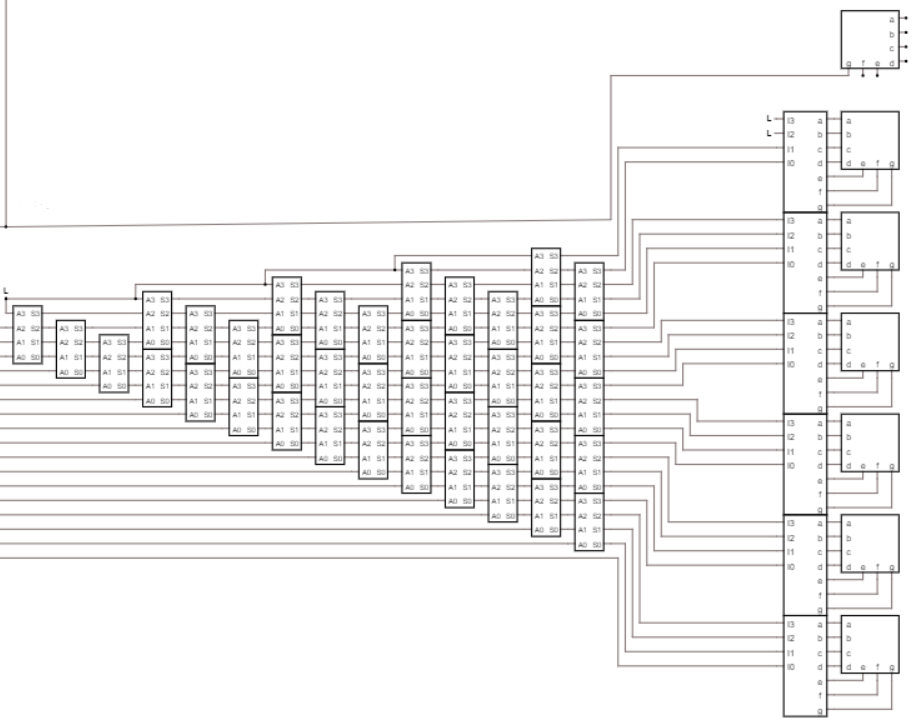
\includegraphics[scale=0.43]{SC_DoubleDabble}
    \caption{Picture of the double dabble, the second part of the circuit}
    \label{DoubleDabble}
  \end{figure}


The algorithm works as follows (graphic representation in figure \ref{SC_Algo}):
\begin{enumerate}
  \item Let's consider a 8-bit binary number, but the same argument works for n bits. 
  \item Let's consider the units, as long as that binary value is lower or equal to 4, the binary input can keep shifting and increasing the units.
  \item When the units value is an integer greater than 4, 3 is added to them and the shifting process continues.
\end{enumerate}

It is mandatory to add 3 because during the conversion the weight of the 4 bits of the unit is 16, at maximum, whereas those for digits represent a maximum of 10 in decimal form. So to compensate this loss, we add a half of the lost weight.

\begin{table}[h]
  \centering
  \begin{tabular}{||c|c|c|c||c||c||}
    \hline
    \# & Hundreds & Tens & Units & Binary & Operation \\
    \hline
    1 & 0000 & 0000 & 0000 & 11111111 & Start \\
    2 & 0000 & 0000 & 0001 & 11111110 & Shift1 (every 4-bit slot < 5) \\
    3 & 0000 & 0000 & 0011 & 11111100 & Shift2 (every 4-bit slot < 5) \\ 
    4 & 0000 & 0000 & 0111 & 11111000 & Shift3 (every 4-bit slot < 5) \\
    5 & 0000 & 0000 & 1010 & 11110000 & Add-3 to "Units" ("Units" $\geq$ 5)\\
    6 & 0000 & 0001 & 0101 & 11110000 & Shift4 (every 4-bit slot < 5) \\
    7 & 0000 & 0001 & 1000 & 11110000 & Add-3 to "Units" ("Units" $\geq$ 5)\\
    8 & 0000 & 0011 & 0001 & 11100000 & Shift5 (every 4-bit slot < 5) \\
    9 & 0000 & 0110 & 0011 & 11000000 & Shift6 (every 4-bit slot < 5) \\
    10 & 0000 & 1001 & 0011& 11000000 & Add-3 to "Tens" ("Tens" $\geq$ 5)\\
    11 & 0001 & 0010 & 0111& 10000000 & Shift7 (every 4-bit slot < 5) \\
    12 & 0001 & 0010 & 1010& 10000000 & Add-3 to "Units" ("Units" $\geq$ 5)\\
    13 & 0010 & 0101 & 0101& 00000000 & Shift8 (every 4-bit slot < 5) \\
    \hline
  \end{tabular}
    \label{SC_Algo}
    \caption{Double dabble algorithm applied to the decimal number 255}

  \end{table}


The goal of the "Shift and add 3" component, programmed using the customizable logic of the simulator, is to operate this shift or addition depending on the 4 inputs given. Its truth table is figure \ref{Add3Table}.

\begin{table}[h]
  \centering
  \begin{tabular}{||c|c||}
    \hline
    Input & Output \\
    \hline
    0000 & 0000 \\
    0001 & 0001 \\
    0010 & 0010 \\ 
    0011 & 0011 \\
    0100 & 0100 \\
    0101 & 1000 \\
    0110 & 1001 \\
    0111 & 1010 \\
    1000 & 1011 \\
    1001 & 1100 \\
    \hline
  \end{tabular}
    \label{Add3Table}
    \caption{"Shift and add 3" truth table}
  \end{table}

It is clear, thanks to this figure, that when the number is greater than four it gets added three to it. The "shift" part can be seen in figure \ref{DoubleDabble}. If we consider the input A0 of a single Add3 component, its output, S0, is the input A1 for the next component.

After all this process the number is divided into 4 bit groups that enter the 7-segment decoders and than display the result on led displays.






\clearpage
\section{Appendix}

\begin{figure}[h]
    \centering
    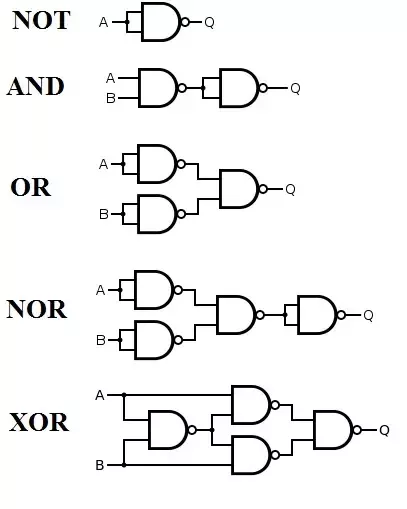
\includegraphics[scale=.42]{IM_NAND_allpowerful.png}
    \caption{NAND gate is functional complete, every other logic gate can be a circuit made of NANDs only}
    \label{NAND_allpowerful}
\end{figure}

\begin{figure}[h]
    \centering
    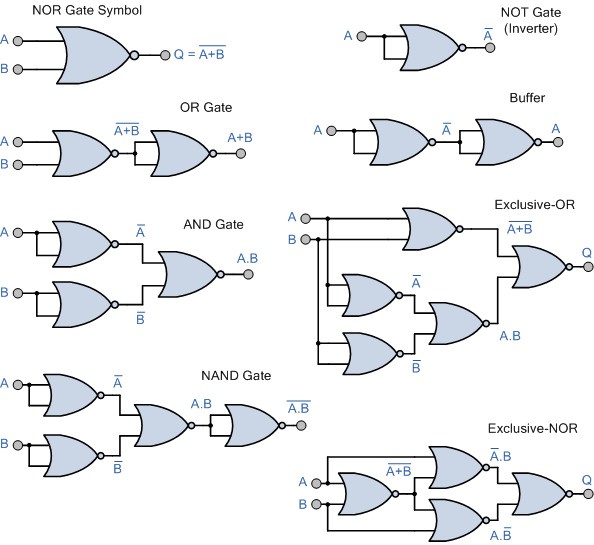
\includegraphics[scale=.5]{IM_NOR_allpowerful.png}
    \caption{NOR gate is functional complete, every other logic gate can be a circuit made of NORs only}
    \label{NOR_allpowerful}
\end{figure}

\begin{figure}[h]
  \centering
  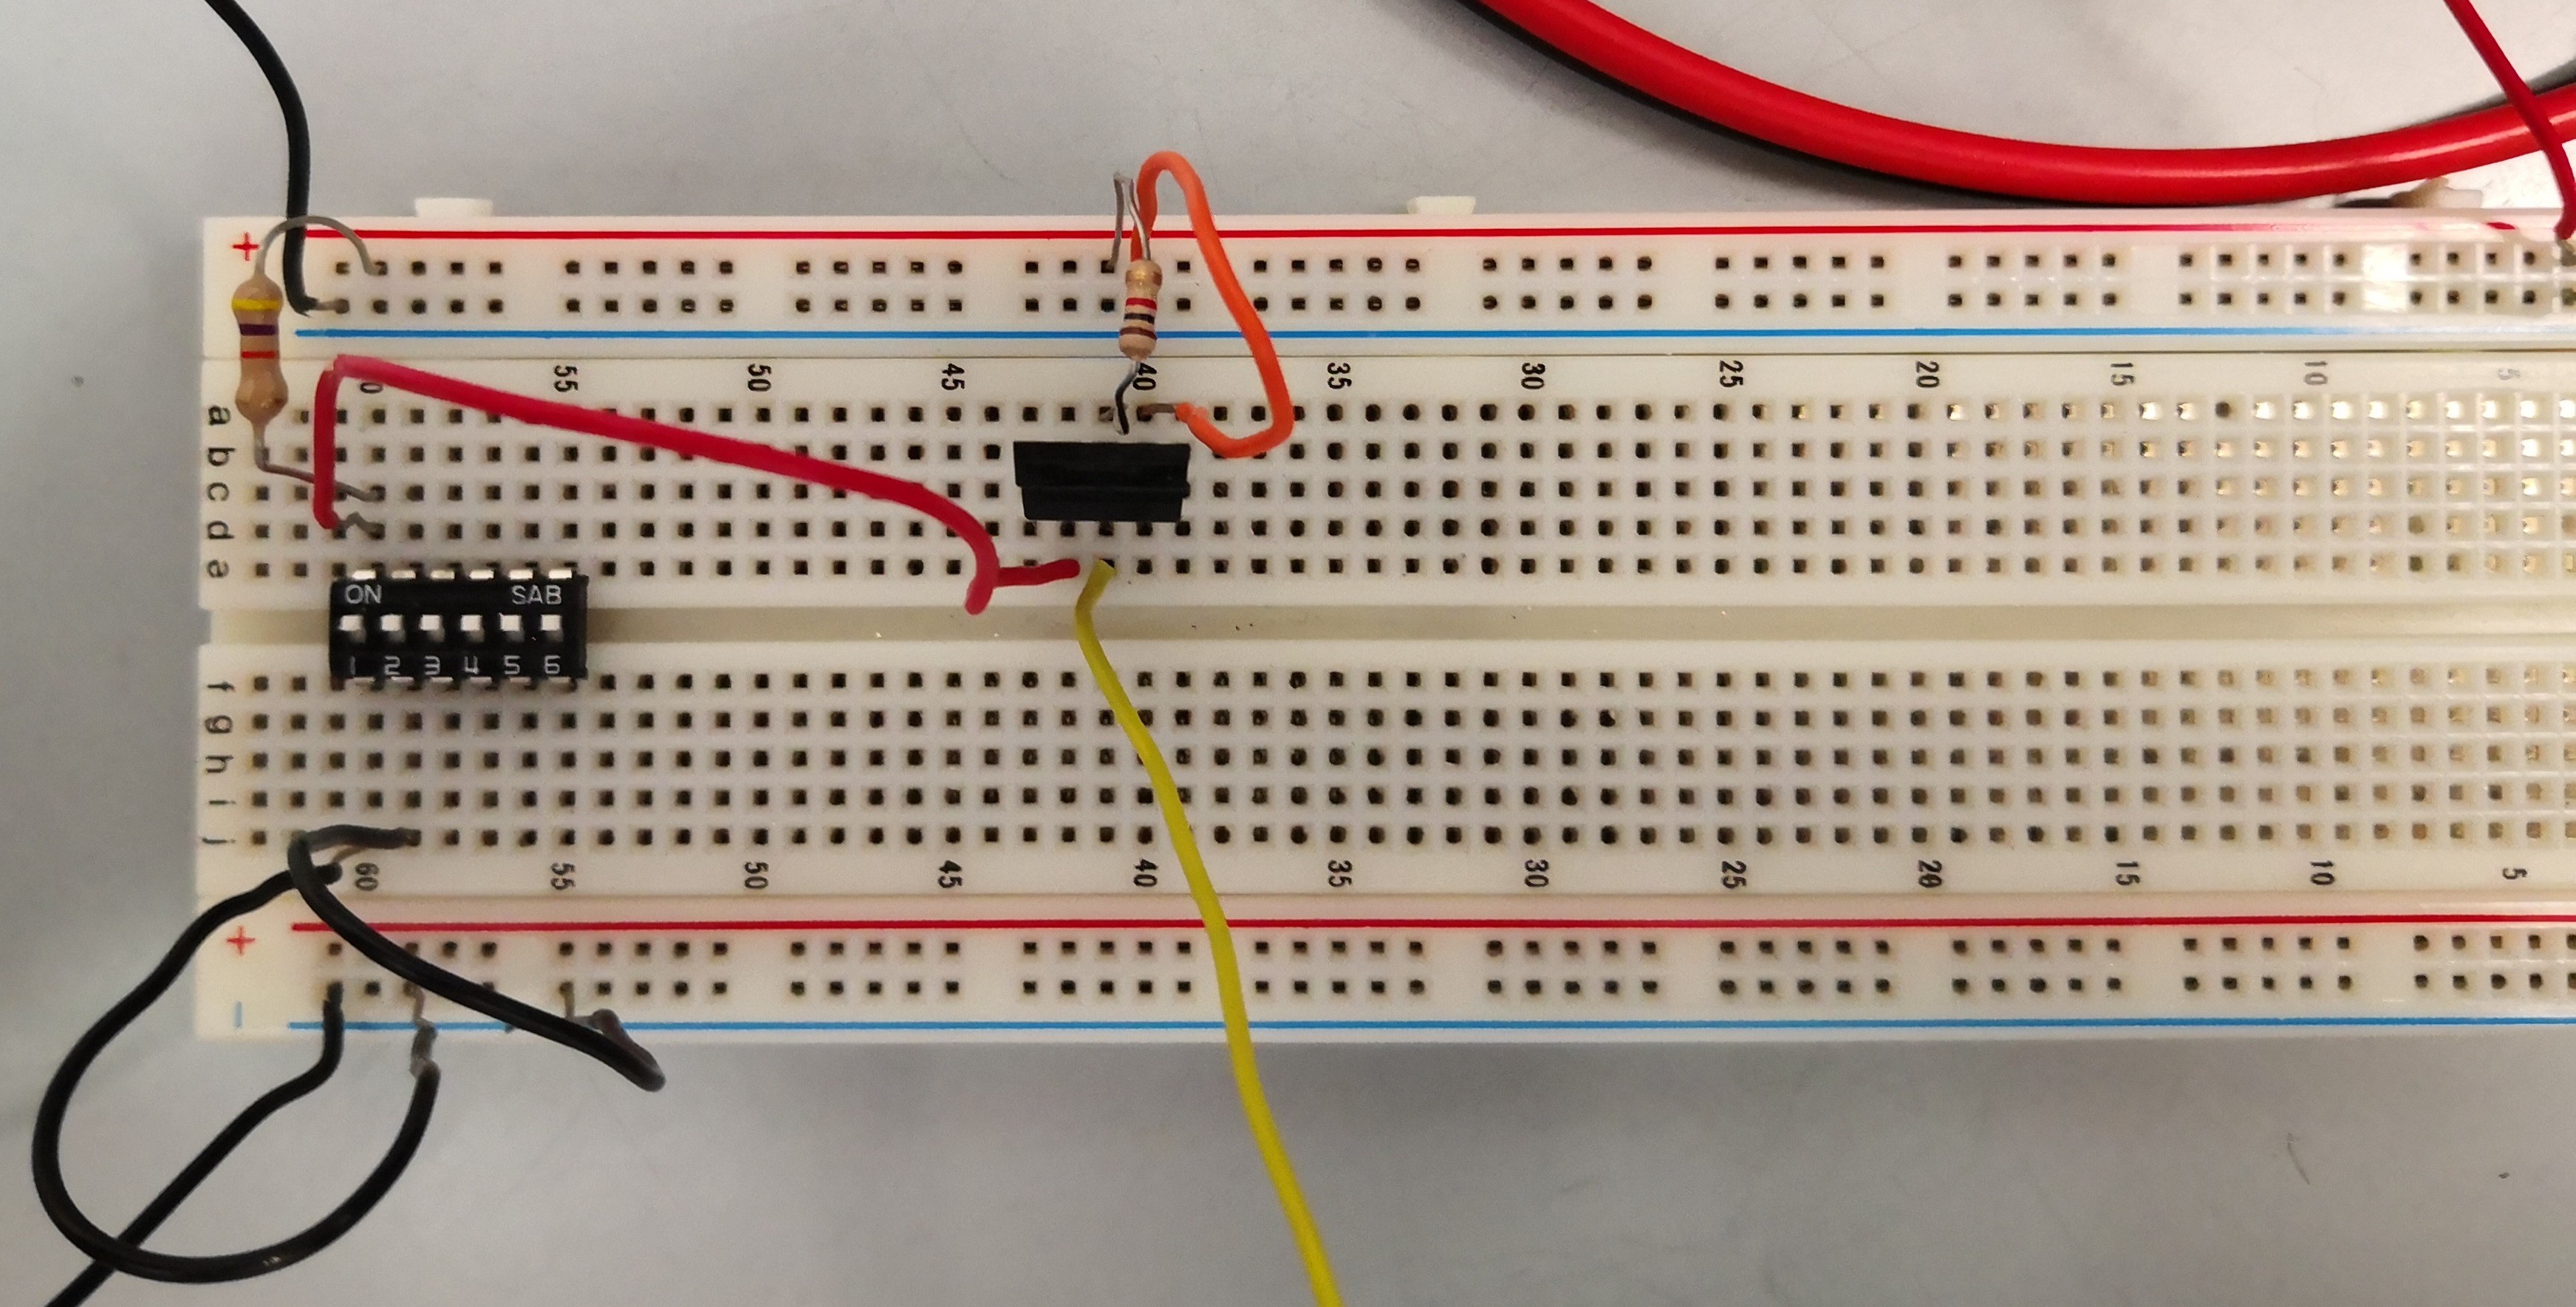
\includegraphics[scale=.08]{IM_NOT_LAB.jpg}
  \caption{NOT gate realized in laboratory}
  \label{NOT_LAB}
\end{figure}

\begin{figure}[h]
  \centering
  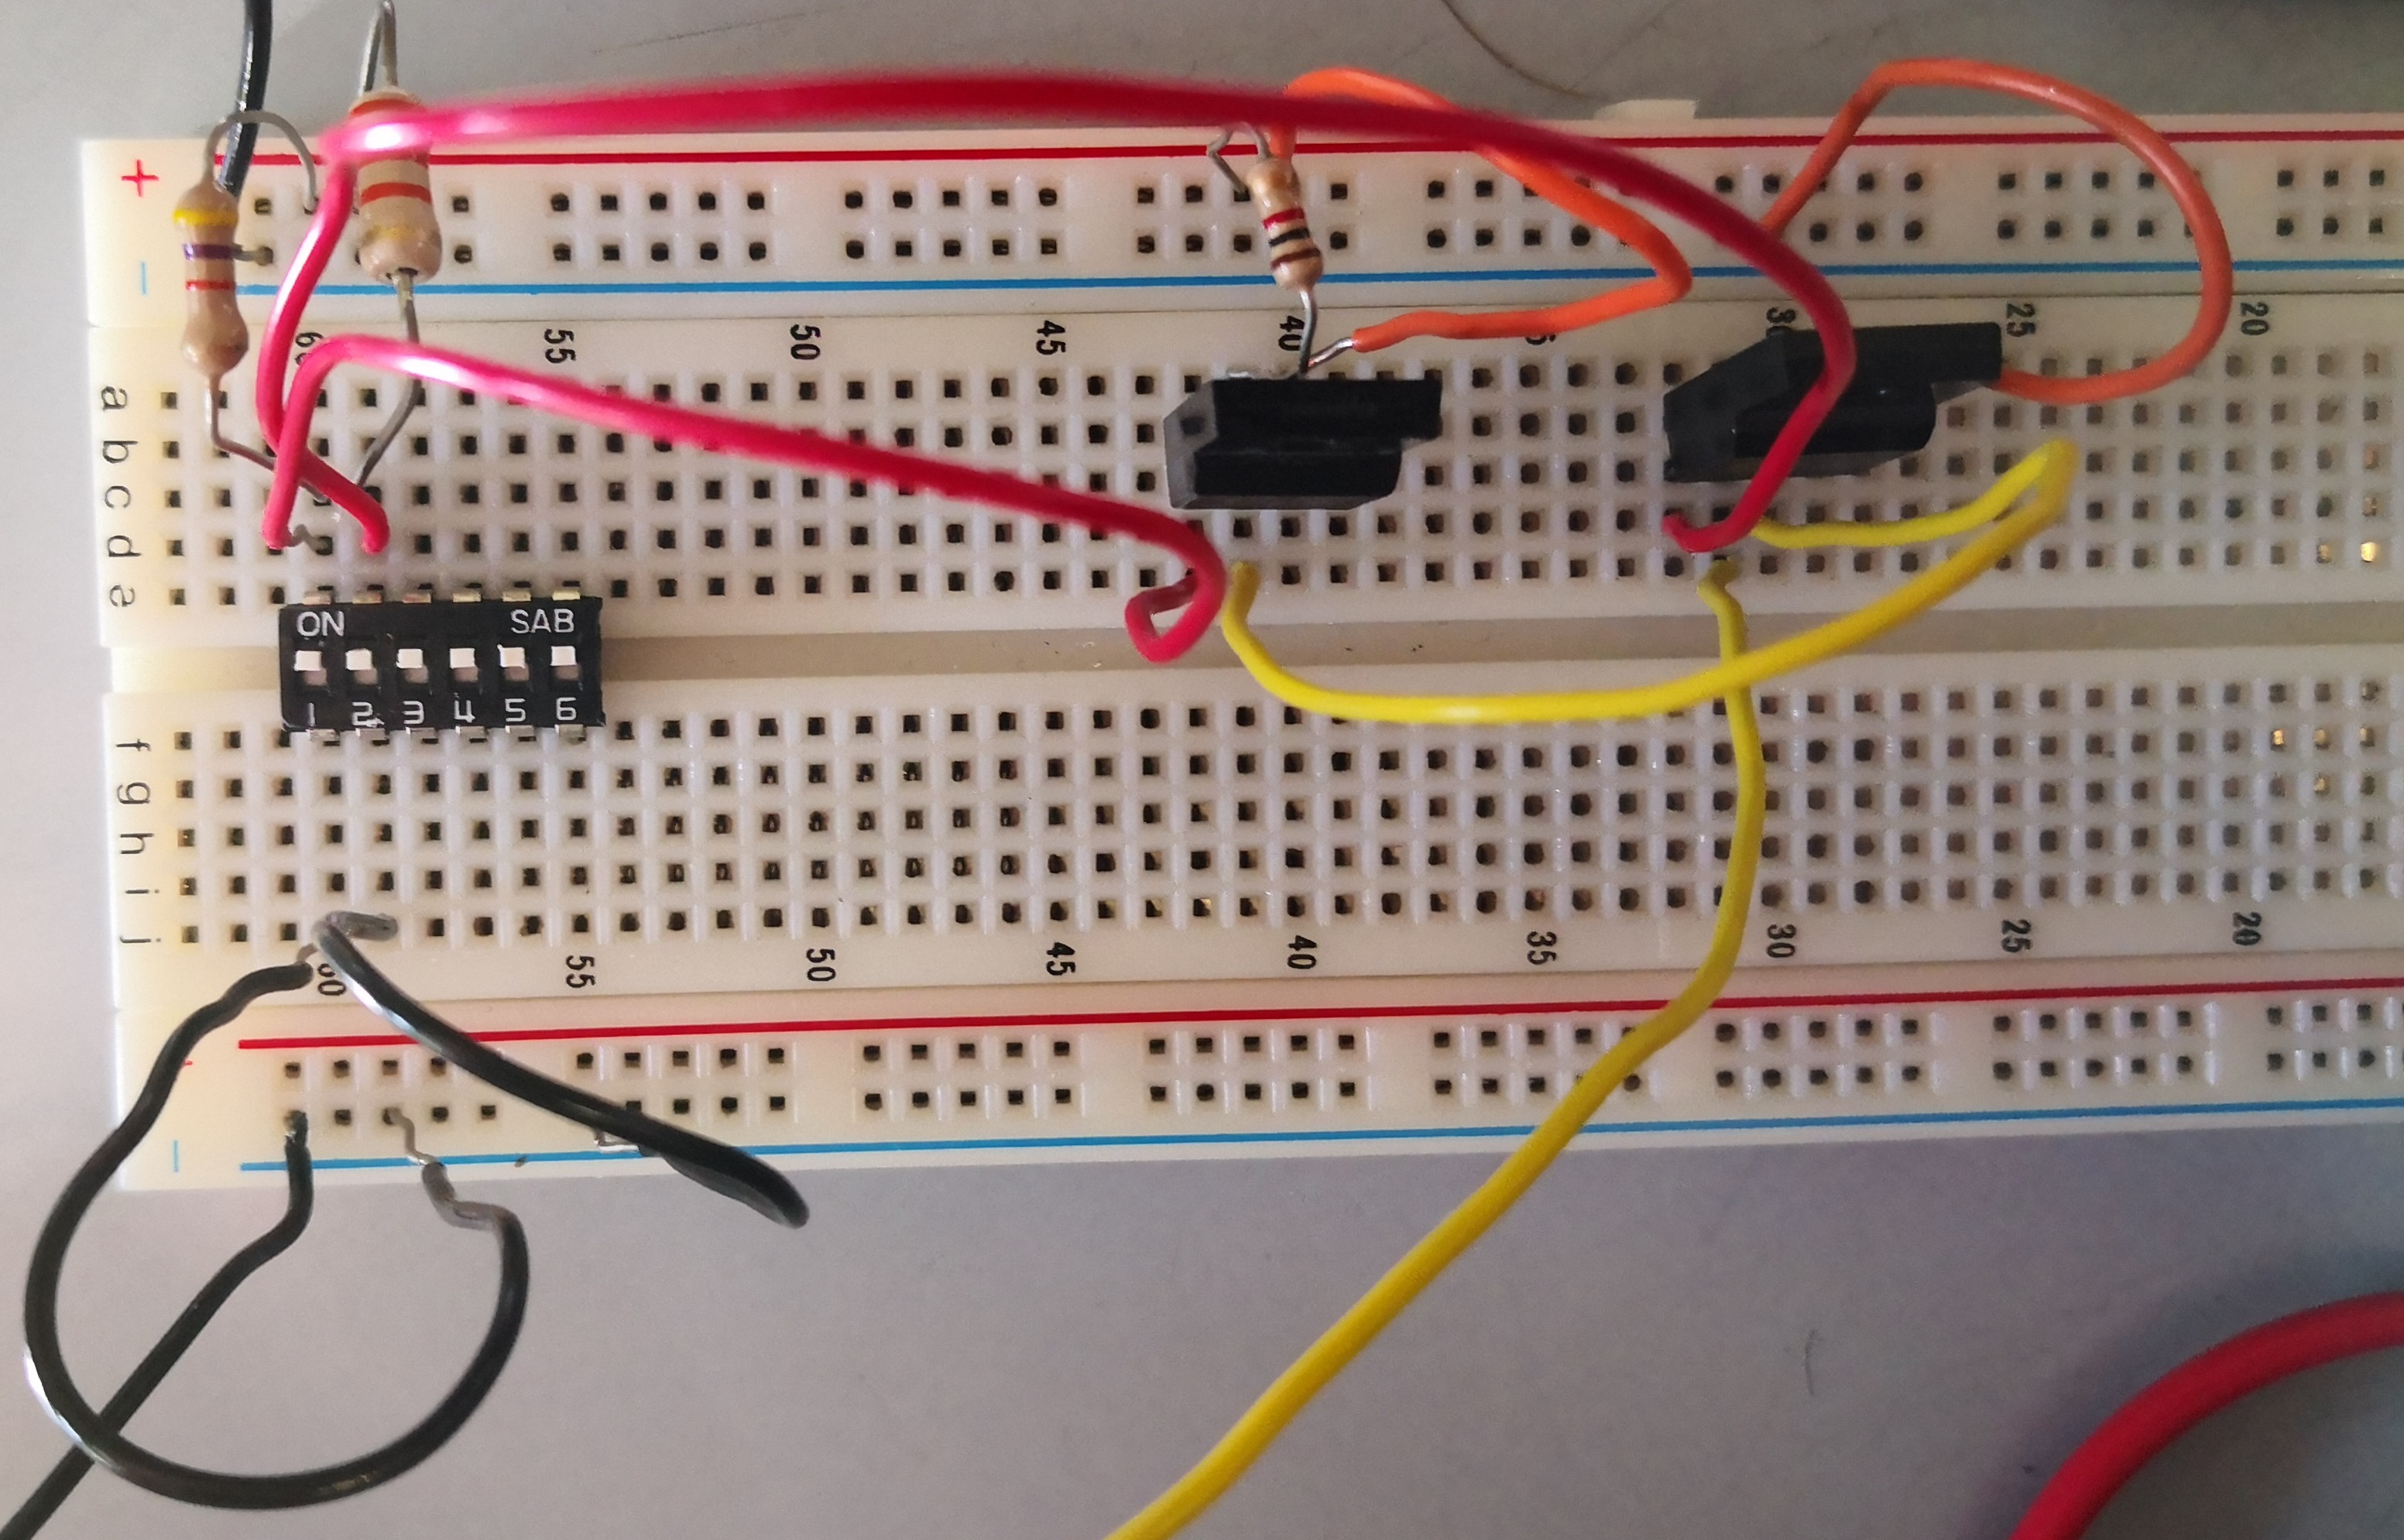
\includegraphics[scale=.08]{IM_NOR_LAB.jpg}
  \caption{NOR gate realized in laboratory}
  \label{NOR_LAB}
\end{figure}

\begin{figure}[h]
  \centering
  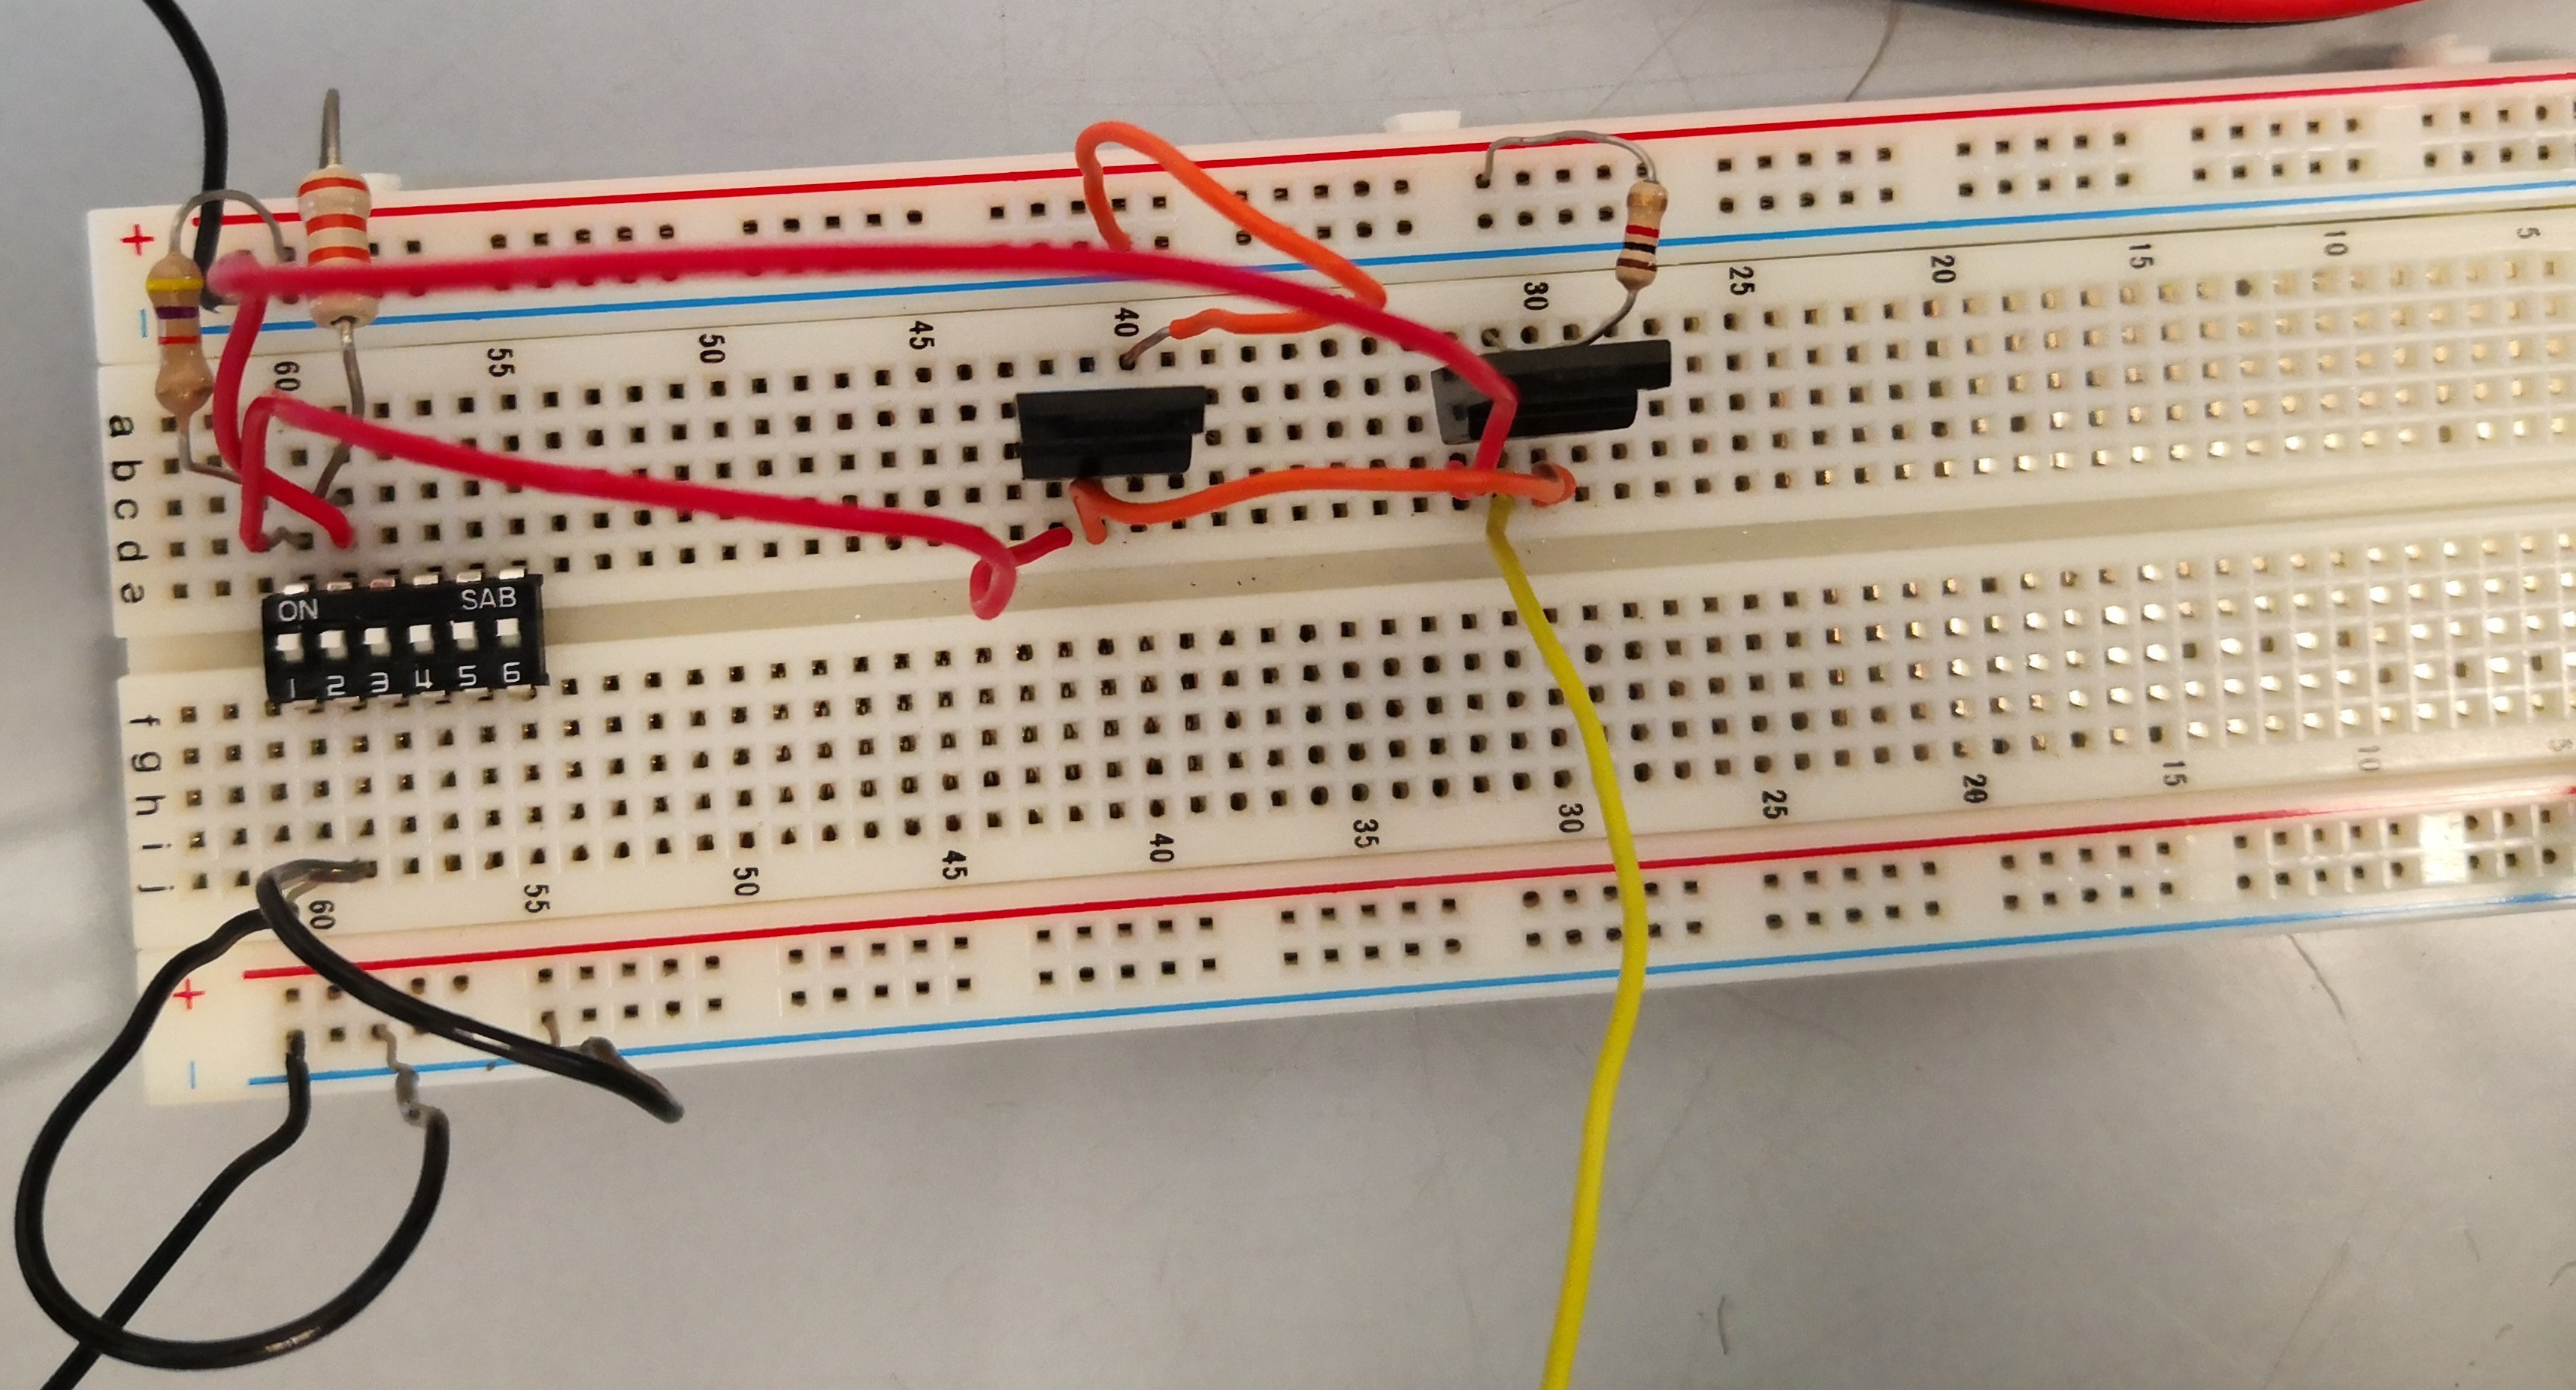
\includegraphics[scale=.08]{IM_NAND_LAB.jpg}
  \caption{NAND gate realized in laboratory}
  \label{NAND_LAB}
\end{figure}




 
\end{document}